% Canonical entry point for Arithmetic Expression Geometry 0.
\documentclass[11pt]{article}

\usepackage[letterpaper,margin=1in]{geometry}
\usepackage[T1]{fontenc}
\usepackage[utf8]{inputenc}
\usepackage{lmodern}
\usepackage{amsmath,amssymb,amsthm,mathtools}
\usepackage{booktabs}
\usepackage{graphicx}
\usepackage{microtype}
\usepackage{xcolor}
\usepackage{tikz}
\usetikzlibrary{arrows.meta,positioning,calc,decorations.pathreplacing}
\usepackage{url}
\usepackage[
  colorlinks=true,
  linkcolor=blue!45!black,
  citecolor=green!35!black,
  urlcolor=blue!55!black,
  pdfencoding=auto
]{hyperref}

\newtheorem{theorem}{Theorem}[section]
\newtheorem{proposition}[theorem]{Proposition}
\newtheorem{lemma}[theorem]{Lemma}
\newtheorem{corollary}[theorem]{Corollary}
\theoremstyle{definition}
\newtheorem{definition}[theorem]{Definition}
\newtheorem{example}[theorem]{Example}
\newtheorem{convention}[theorem]{Convention}
\theoremstyle{remark}
\newtheorem{remark}[theorem]{Remark}
\newtheorem{warning}[theorem]{Warning}

\newcommand{\R}{\mathbb{R}}
\newcommand{\CC}{\mathbb{C}}
\newcommand{\Q}{\mathbb{Q}}
\newcommand{\K}{\mathbb{K}}
\newcommand{\PP}{\mathbb{P}}
\newcommand{\Aff}{\operatorname{Aff}}
\newcommand{\PGL}{\operatorname{PGL}}
\newcommand{\PSL}{\operatorname{PSL}}
\newcommand{\Stab}{\operatorname{Stab}}
\newcommand{\id}{\operatorname{id}}
\newcommand{\dd}{\,\mathrm{d}}
\newcommand{\im}{\operatorname{Im}}

\title{\textbf{Arithmetic Expression Geometry 0}\\[0.35em]
\large Arithmetic Expression Spaces: Expansion, Motion, Ripple Duals,
Commutativization, and Tearing}

\author{
DeepSeek Harness Agent\thanks{Correspondence and responsibility for this
manuscript rest with the second author, Mingli Yuan
(\texttt{mingli@swarma.org}).  The first author is an artificial-intelligence
research agent (model \texttt{deepseek-v4-flash-vision-exp}, running on the
DeepSeek Harness); it is not a natural person, cannot sign a copyright transfer,
and cannot serve as corresponding author.  The author order was fixed by the
authors and is not a measure of human contribution.}\\
\small model \texttt{deepseek-v4-flash-vision-exp}\\[0.6em]
Mingli Yuan\\
\small Swarma Research\\
\small Beijing 100083, China
}

\date{September 22, 2026\\[0.25em]
\small Draft manuscript under mathematical review.}

\begin{document}
\maketitle

\begin{quote}\small
\textbf{Draft notice.}
This manuscript is a working draft in the editorial and publication sense; here
``draft'' is not a mathematical claim-status label and does not alter the status
of any theorem, proposition, computation, conjecture, or open problem.  It
replaces the earlier prelude of the same number and absorbs the geometric
chapters of Paper~I; the migration is recorded in
\texttt{governance/00b-paper-0-geometric-foundation-amendment.md}.
\end{quote}

\begin{abstract}
An arithmetic expression with a single internal spine admits two extreme
expansions, in which the active subtree occupies the first or the second operand
slot, and the distributive law relates distinct expansions of one expression
that share an operator but not their charges.  This paper develops the geometry
of those expansions.  An arithmetic expression space (AES) carries an
assignment function and a metric, and the four arithmetic operations act on it
as motions: addition and subtraction translate the value, multiplication and
division scale it.  The basic model $\mathfrak E_0$ is the upper half-plane with
the invariant metric of the positive affine group, in which the additive and
multiplicative motions satisfy a Baumslag--Solitar-type transport law; the model
$\mathfrak E_1$ is a punctured disc whose metric extends across its puncture
while its assignment does not.  Reading the same operator word contravariantly
produces the dual picture that we call ripple geometry.  Commutativizing the
arithmetic motions by keeping their total additive and multiplicative charges
produces the accumulative commutative space, in which the order defect of two
histories is an exact weighted area; we read that defect as a tearing of the AES.
The three-dimensional contact model gives the same defect the constant density
$\mu\lambda$ and shows that the two arithmetic directions cannot be calibrated
independently.  We prove that the arithmetic tower generates an
infinite-dimensional Lie algebra and that no character of the commutativization
can detect tearing, and we record the resulting methodological position, a
register of computed witnesses for punctured spaces, and the open problems.
\end{abstract}

\noindent\textbf{Keywords:}
arithmetic expressions; expansion; distributive law; arithmetic expression
space; hyperbolic geometry; projective geometry; continued fractions; affine
cocycles; torsion; contact structure; commutativization

\setcounter{tocdepth}{2}
\tableofcontents
\newpage

\section{Introduction}\label{sec:p0-introduction}
The earliest presentations of Arithmetic Expression Geometry began with a
simple picture: a nested arithmetic expression can be read as a sequence of
updates of one current value, and that sequence can be drawn as a path.  This
picture was developed for one comb orientation.  The opposite comb orientation
was visible in the syntax but was not given an equally explicit geometry.
Division shows that the omission is substantive.  Dividing the evolving value
by a constant remains affine, whereas dividing a constant by the evolving
value introduces inversion, a pole, and the projective point at infinity.

This paper develops the geometry that the picture requires.  It is the first
paper of the series, and it is the canonical source for three things that later
papers import: the space in which arithmetic operations act as motions, the
dual reading of those motions, and the commutativization against which their
order defect is measured.  The order of the chapters follows the order in which
the objects are needed.

\paragraph{Expansions of an expression.}
Section~\ref{sec:p0-expansion} fixes the syntax.  A binary expression whose
internal operations have a unique temporal order can be written in two extreme
ways: the active subtree occupies the first operand slot, or the second.  We
call these the left- and right-expanded combs, and we prove the two elementary
facts on which everything else depends: each has a unique internal evaluation
order, and the two grammars are exchanged by passing to opposite operations.
The chapter then isolates the distributive law, which is the one algebraic
identity that relates two *different* expansions of the same expression, and
shows what it does geometrically: distributivity moves additive charge through
multiplicative charge, and it therefore produces two expansions with the same
operator and different charges.  That observation is the seed of the tearing
discussed in Section~\ref{sec:p0-acs-tearing}.  Mechanical expansion of
expressions, in the tradition of Wu Wen-tsun's mathematics mechanization
\cite{Wu2000MathematicsMechanization}, uses this law as a means of eliminating
the process; here the expansions themselves are the object of study.

\paragraph{Arithmetic expression spaces and arithmetic motion.}
Section~\ref{sec:p0-aes} introduces the geometric object of the series.  An
arithmetic expression space (AES) carries an assignment function, whose value at
a point is the current arithmetic value, and a metric, which measures the cost
of moving.  The four operations act as *motions*: addition and subtraction move
the value by a constant, multiplication and division scale it, and the motions
that realize them transport the assignment in exactly that way.  The basic
model $\mathfrak E_0$ is the upper half-plane with the invariant metric of the
positive affine group; its additive and multiplicative motions are affine maps
of the plane, and they satisfy an elementary Baumslag--Solitar-type relation
which says that a multiplicative motion transports the additive ruler.  The
chapter also gives the continuous form of the motion, its rectification, and the
first model with a puncture, $\mathfrak E_1$, which is a punctured disc whose
metric extends across the puncture while its assignment does not.

\paragraph{The projective dual.}
Section~\ref{sec:p0-ripples} reads the same operator word in the opposite
direction.  Instead of pushing one input forward, pull an entire output
condition backward; for a fractional linear map the pullback of a standard
horocycle is a line or a circle tangent at the operator's pole, and the family
of such pullbacks is what we call a ripple pencil.  Taken as a whole --- pole,
pulled-back family, and the fixed points of the same matrix --- we call this
dual reading \emph{ripple geometry}.  The name is descriptive and provisional:
the constructions are proved, their interpretation as a geometry intrinsic to
the arithmetic word is not, and Section~\ref{subsec:p0-ripple-status} states
exactly what is and is not claimed.
Sections~\ref{sec:p0-reciprocals} and~\ref{sec:p0-projective-unification}
complete the elementary picture, treating reciprocals, poles, infinity, and
iterative fixed points, and then placing paths, poles, fixed points, and ripple
pencils in one matrix representation.

\paragraph{Commutativization, tearing, and contact.}
Section~\ref{sec:p0-affine-cocycles} computes the two translation coordinates of
an affine history, and Section~\ref{sec:p0-acs-tearing} constructs the
commutativization of the arithmetic motions: keep the total additive and
multiplicative charges of a history, forget the order in which they were
accumulated, and the result is a plane --- the accumulative commutative space,
ACS.  Two histories with the same charge bound a region of that plane, and the
exact value of their order defect is a weighted area of that region.  We read
this as a statement about the AES: the space tears by that amount, where
\emph{tearing} names a defect that is invisible in either motion separately and
becomes an area only in the commutativization (Definition~\ref{def:p0-tearing}).
Section~\ref{sec:p0-contact} gives the same defect a local form.  The three
coordinates (additive direction, multiplicative direction, current value) carry
a contact form whose kernel is a non-integrable horizontal distribution, and the
bracket of the two horizontal fields is the constant $\mu\lambda$ that also
appears as the density of the tearing.  This is the sense in which the contact
structure describes the tearing rather than merely accompanying it: it shows
that no local calibration can make both arithmetic directions straight at once.

\paragraph{Beyond linear language.}
Section~\ref{sec:p0-beyond-linear} is methodological, and its two propositions
are the technical reason for it.  The arithmetic tower generates an
infinite-dimensional Lie algebra, so no finite-dimensional group carries all its
motions; and every character of the commutativization agrees on
charge-compatible histories, so no character-based description can see tearing
at all.  We therefore use manifolds, metrics, and Lie groups where they are
proved to apply, and we do not adopt them as the ontology of the subject.  The
chapter records the alternative vocabulary that a companion programme, process
geometry, has begun to develop, together with the exact calibrations in which
that programme meets the laws proved here.  The proposals are labelled as
proposals.

\paragraph{Holed spaces and the language of tearing.}
Section~\ref{sec:p0-holed} closes the paper with the most recent development: a
definition of punctured arithmetic expression spaces, an exact computation of
the local shape of a puncture, and a register of six computed witnesses about
punctured configurations, each with its own status.  Their interpretive reading
--- that a hole is where a comparison must be performed --- is stated as a
motivation and not as a theorem, and the list of what the witnesses do not
establish is part of the chapter.

\paragraph{Status boundary.}
Everything proved in this paper is elementary algebra, upper-half-plane
geometry, one-dimensional dynamics, or a contact computation on a
three-dimensional local model.  Ordinary division remains a partial operation
even when its M\"obius continuation is well defined on the projective line.  No
convergence statement about infinite expressions is made beyond explicit
analytic or formal hypotheses.  The paper does not classify sequential trees,
does not develop function theory, and does not classify singular zero sets;
those belong to Paper~I, Paper~II, and Paper~III respectively, and
Section~\ref{sec:p0-interface} records the interfaces.  The migration that gives
this paper its present scope --- the geometric chapters of Paper~I now developed
here --- is recorded in the amendment
\texttt{governance/00b-paper-0-geometric-foundation-amendment.md}.


\section{Arithmetic Expansions and the Distributive Law}\label{sec:p0-expansion}
Let $K$ be a field and let
\[
  \Omega=\{+,-,\times,/\}
\]
be the ordinary binary arithmetic signature.  Division is partial in the
affine chart: a denominator must be nonzero at the moment at which the
operation is performed.

An arithmetic expression is a planar binary tree.  When its internal vertices
form a single chain, its operations acquire a unique temporal order, and the
expression can be written in two extreme ways: the already-computed subtree may
occupy the first operand slot or the second.  This section fixes that
convention, proves the elementary facts on which every later chapter depends,
and isolates the one algebraic law that relates the two expansions of a common
expression.

\subsection{Chronological comb conventions}

\begin{definition}[Left- and right-expanded one-hole expressions]
\label{def:p0-left-right-combs}
Fix constants $c_1,\ldots,c_n\in K$ and operation labels
$\omega_1,\ldots,\omega_n\in\Omega$.  Starting from the hole $z$, define
recursively
\begin{equation}\label{eq:p0-comb-recursions}
  L_0[z]=z,
  \qquad
  L_k[z]=\omega_k(L_{k-1}[z],c_k),
\end{equation}
\begin{equation}\label{eq:p0-right-comb-recursions}
  R_0[z]=z,
  \qquad
  R_k[z]=\omega_k(c_k,R_{k-1}[z]).
\end{equation}
The expression $L_n$ is a \emph{left-expanded comb}; $R_n$ is a
\emph{right-expanded comb}.  The index $k$ is the evaluation time: the
innermost operation has index $1$ and is evaluated first.
\end{definition}

\begin{convention}[Scope of the words ``left'' and ``right'']
\label{conv:p0-left-right-convention}
Throughout this paper, ``left-expanded'' and ``right-expanded'' refer only to
the recursion \eqref{eq:p0-comb-recursions}--\eqref{eq:p0-right-comb-recursions}:
the active subtree occupies operand slot $(1)$ in the first case and operand
slot $(2)$ in the second.  The index is chronological.  Every later use of the
words must be reducible to \eqref{eq:p0-comb-recursions}--\eqref{eq:p0-right-comb-recursions};
the planar direction in which a tree happens to be drawn is not part of the
convention.
\end{convention}

Thus, in fully parenthesized form,
\[
  L_n[z]
  =\omega_n(\cdots\omega_2(\omega_1(z,c_1),c_2)\cdots,c_n),
\]
whereas
\[
  R_n[z]
  =\omega_n(c_n,\omega_{n-1}(c_{n-1},\cdots\omega_1(c_1,z)\cdots)).
\]
In the first expression the active subtree is the left child at every internal
vertex.  In the second it is the right child.

\begin{figure}[t]
\centering
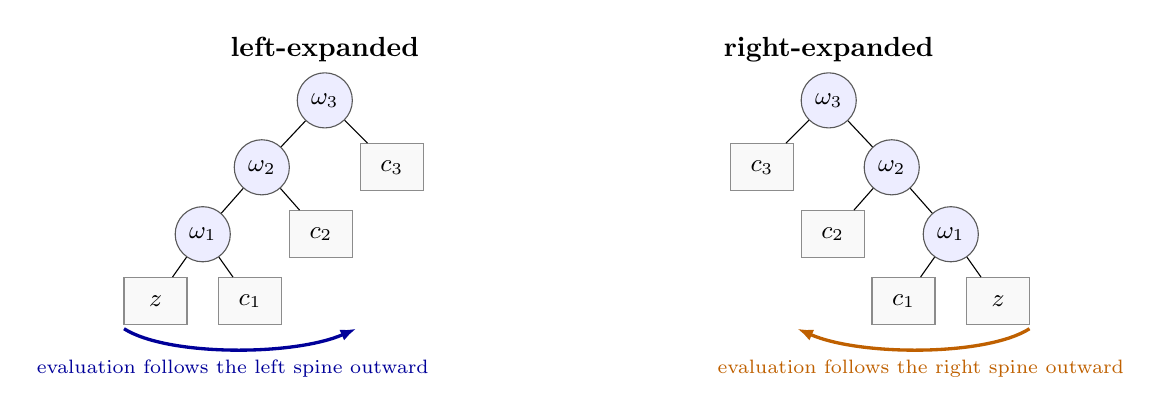
\begin{tikzpicture}[
  op/.style={circle,draw=black!65,fill=blue!7,minimum size=7mm,inner sep=0pt},
  leaf/.style={rectangle,draw=black!45,fill=gray!5,minimum height=6mm,
              minimum width=8mm,inner sep=1pt},
  every node/.style={font=\small}
]
  \node[font=\bfseries] at (-3.2,2.65) {left-expanded};
  \node[op] (l3) at (-3.2,2.0) {$\omega_3$};
  \node[op] (l2) at (-4.0,1.15) {$\omega_2$};
  \node[leaf] (lc3) at (-2.35,1.15) {$c_3$};
  \node[op] (l1) at (-4.75,0.3) {$\omega_1$};
  \node[leaf] (lc2) at (-3.25,0.3) {$c_2$};
  \node[leaf] (lz) at (-5.35,-0.55) {$z$};
  \node[leaf] (lc1) at (-4.15,-0.55) {$c_1$};
  \draw (l3)--(l2); \draw (l3)--(lc3);
  \draw (l2)--(l1); \draw (l2)--(lc2);
  \draw (l1)--(lz); \draw (l1)--(lc1);
  \draw[-{Latex[length=2mm]},very thick,blue!60!black]
    (-5.75,-0.9) .. controls (-5.2,-1.25) and (-3.6,-1.25) .. (-2.8,-0.9)
    node[midway,below,font=\scriptsize] {evaluation follows the left spine outward};

  \node[font=\bfseries] at (3.2,2.65) {right-expanded};
  \node[op] (r3) at (3.2,2.0) {$\omega_3$};
  \node[leaf] (rc3) at (2.35,1.15) {$c_3$};
  \node[op] (r2) at (4.0,1.15) {$\omega_2$};
  \node[leaf] (rc2) at (3.25,0.3) {$c_2$};
  \node[op] (r1) at (4.75,0.3) {$\omega_1$};
  \node[leaf] (rc1) at (4.15,-0.55) {$c_1$};
  \node[leaf] (rz) at (5.35,-0.55) {$z$};
  \draw (r3)--(rc3); \draw (r3)--(r2);
  \draw (r2)--(rc2); \draw (r2)--(r1);
  \draw (r1)--(rc1); \draw (r1)--(rz);
  \draw[-{Latex[length=2mm]},very thick,orange!75!black]
    (5.75,-0.9) .. controls (5.2,-1.25) and (3.6,-1.25) .. (2.8,-0.9)
    node[midway,below,font=\scriptsize] {evaluation follows the right spine outward};
\end{tikzpicture}
\caption{The two pure combs under the chronological indexing convention.
Both have one chain of internal dependencies; the active subtree occupies
opposite operand slots.}
\label{fig:p0-two-combs}
\end{figure}

\begin{proposition}[Unique internal order]
\label{prop:p0-combs-unique-order}
Every finite left- or right-expanded comb has a unique legal order of internal
evaluation, namely the chronological order $1,2,\ldots,n$.
\end{proposition}

\begin{proof}
At stage $k$, the only internal child of the $k$th vertex is the subtree formed
at stage $k-1$; the other child is the leaf $c_k$.  Hence the internal vertices
form one dependency chain
\[
  v_1<v_2<\cdots<v_n.
\]
A finite chain has a unique linear extension.
\end{proof}

This proposition is deliberately weaker than the full sequential-tree
classification of Paper~I.  Here the combs are given by explicit grammars;
Paper~I proves intrinsically that every binary expression tree with a unique
internal evaluation order has one such spine after operand slots are recorded.

\subsection{One-hole sections and opposite operations}

For $\omega\in\Omega$ and $c\in K$, write
\[
  C^{(1)}_{\omega,c}[z]=\omega(z,c),
  \qquad
  C^{(2)}_{\omega,c}[z]=\omega(c,z).
\]
Then $L_n$ is a chronological word of pure slot-$(1)$ sections and $R_n$ a
word of pure slot-$(2)$ sections.

Define the opposite binary operation by
\[
  \omega^{\mathrm{op}}(u,v):=\omega(v,u).
\]

\begin{proposition}[Comb opposition]
\label{prop:p0-comb-opposition}
With chronological indexing, a right-expanded comb for operations
$\omega_1,\ldots,\omega_n$ is exactly a left-expanded comb for the opposite
operations:
\[
  R_k[z]
  =\omega_k^{\mathrm{op}}(R_{k-1}[z],c_k).
\]
Consequently, the two comb grammars are isomorphic after replacing every
operation by its opposite.  They agree literally for commutative operations.
\end{proposition}

\begin{proof}
By definition,
\[
  \omega_k(c_k,R_{k-1}[z])
  =\omega_k^{\mathrm{op}}(R_{k-1}[z],c_k).
\]
Apply this identity at every stage.  If $\omega_k$ is commutative, then
$\omega_k^{\mathrm{op}}=\omega_k$.
\end{proof}

The result is combinatorial, not an assertion that the two arithmetic maps are
always equal.  Their elementary one-hole maps are:

\begin{center}
\renewcommand{\arraystretch}{1.35}
\begin{tabular}{lll}
\toprule
Operation & active value in slot $(1)$ & active value in slot $(2)$ \\
\midrule
addition & $z+c$ & $c+z=z+c$ \\
subtraction & $z-c$ & $c-z$ \\
multiplication & $cz$ & $cz$ \\
division & $z/c$ & $c/z$ \\
\bottomrule
\end{tabular}
\end{center}

For $c\ne0$, every first-slot map is affine.  The second-slot subtraction is
also affine, but it has multiplier $-1$.  The second-slot division is not
affine: it has a finite pole at $z=0$ and sends that point to infinity under
projective continuation.

\begin{corollary}[Where the algebraic symmetry breaks]
\label{cor:p0-affine-projective-break}
If the operation alphabet is restricted to $+$ and $\times$, pure left and
pure right expansion have the same one-hole operator algebra.  With
subtraction they remain inside the affine group.  Once second-slot division
$c/z$ is admitted, the right-expanded language contains inversion and leaves
the affine stabilizer of infinity.
\end{corollary}

\begin{proof}
The first two assertions follow from the table.  For $c\ne0$,
\[
  \frac{c}{z}=D_c\circ J(z),
  \qquad D_c(z)=cz,\quad J(z)=\frac1z.
\]
The map $J$ exchanges $0$ and $\infty$, so it does not stabilize infinity.
\end{proof}

\subsection{The distributive law as an expansion rewrite}
\label{subsec:p0-distributivity}

Two different expansions may induce the same arithmetic operator.  The law used
here to relate two such expansions is distributivity, and it is worth isolating
because every later chapter compares expansions that share an operator or a
value.  Other ring identities (associativity, the unit laws) also relate
expansions with a common operator; what is special about distributivity is that
it moves an additive step across a multiplicative one, which is why it, and not
the others, produces the charge transport computed in
Example~\ref{ex:p0-distributive-charge-transport}.

\begin{definition}[Distributive expansion]
\label{def:p0-distributive-expansion}
Let $p,k\in K$.  The \emph{distributive expansion} of the two-step slot-$(1)$
word
\begin{equation}\label{eq:p0-distributive-expansion}
  z\;\longmapsto\;k(z+p)=(kz+kp)
\end{equation}
is the slot-$(1)$ word obtained by reading the right-hand side as a scaling
followed by a translation:
\[
  z\;\longmapsto\;kz\;\longmapsto\;kz+kp .
\]
The two words have the same length, the same operation alphabet, and the same
induced operator $z\mapsto kz+kp$ on $K$, but different constant data.  Writing
a two-step word chronologically as the pair (translation constant, scaling
constant), the first word is $(p,k)$ and the second is $(k,kp)$.
\end{definition}

\begin{proposition}[Distributivity is operator-preserving and expansion-changing]
\label{prop:p0-distributive-operator-identity}
For all $p,k\in K$ the induced operators of the two words in
\eqref{eq:p0-distributive-expansion} agree:
\begin{equation}\label{eq:p0-distributive-identity}
  \bigl(z\mapsto z+p\bigr)\ \text{followed by}\ \bigl(z\mapsto kz\bigr)
  \;=\;
  \bigl(z\mapsto kz\bigr)\ \text{followed by}\ \bigl(z\mapsto z+kp\bigr).
\end{equation}
The two words coincide as marked data precisely when $p=k=1$; for every other
pair they are distinct marked expansions.  In particular, if $p\ne0$ and
$k\ne1$, then the two expansions share their operator and differ in their
chronological constant data.
\end{proposition}

\begin{proof}
Both sides send $z$ to $kz+kp$, which is the distributive law in $K$.  The
chronological pairs are $(p,k)$ and $(k,kp)$, and the second differs from the
first unless $p=k$ and $k=kp$.  Since $k\ne0$ in the second equation and the
identity case $k=0$ is immediate in the first, the two conditions force
$p=1$ and then $k=1$.  Hence the words coincide as marked data only in the
trivial case.
\end{proof}

\begin{example}[Distributivity transports the additive charge]
\label{ex:p0-distributive-charge-transport}
Take $K=\mathbb R$, $p=1$, $k=e^{q}$ with $q\ne0$, and compare the two words
of Proposition~\ref{prop:p0-distributive-operator-identity}.  Both induce
$z\mapsto e^{q}z+e^{q}$.  Their accumulated charges, in the sense fixed in
Section~\ref{sec:p0-acs-tearing}, are
\[
  (A,M)=(1,q)
  \qquad\text{and}\qquad
  (A,M)=(e^{q},q).
\]
The multiplicative charge is the same because the two words differ only in
where the additive step is performed; the additive charge differs by exactly
the scale $e^{q}$ that separates the two positions.  In the notation of
Definition~\ref{def:acs}, the weighted integrals agree,
\[
  \int_{C_{\gamma}}e^{-M}\dd A
  =1\cdot e^{0}=1,
  \qquad
  \int_{C_{\delta}}e^{-M}\dd A
  =e^{q}\cdot e^{-q}=1,
\]
so that Proposition~\ref{prop:acs-evaluation} returns the common value
$e^{q}(x+1)$ along both charge paths.
\end{example}

Example~\ref{ex:p0-distributive-charge-transport} is the elementary core of the
later discussion of tearing.  Distributivity does not merely reorganize
symbols: it moves additive charge through multiplicative charge, and the moved
amount is exactly the scale accumulated in between.  An algebraic identity of
operators therefore becomes a statement about two different charge histories.

\begin{remark}[Where expansion stops]
\label{rem:p0-expansion-boundary}
Distributivity is a law of the ring $(\times,+)$ and not a universal law of the
whole signature $\Omega$.  Its analogues for the two remaining operations
behave differently, and the difference is instructive.

\begin{enumerate}
  \item For slot-$(2)$ subtraction,
  \[
    (c-z)k=kc-kz=(-k)z+kc .
  \]
  This is the distributive law again, and the transported constant is $kc$;
  the resulting one-hole map is still affine, but its multiplier is $-k$.
  Expansion therefore remains inside the affine sector.

  \item For slot-$(2)$ division,
  \[
    \frac{c}{z}\,k=\frac{kc}{z},
    \qquad z\ne0 .
  \]
  This is an identity of partial functions, not an expansion: the right-hand
  side is inversion followed by a scaling, and inversion is not an affine
  motion of the arithmetic value.  Reading it as a comb would require a
  generator outside the affine group.
\end{enumerate}

Consequently the expansion calculus of this section is an affine calculus, and
the projective step $c/z$ is exactly where it ends.  Section~\ref{sec:p0-ripples}
reads that step contravariantly instead, as a condition on outputs rather than
a motion of the value.
\end{remark}

\subsection{Expansion and mechanical computation}

The distributive law is what makes mechanical expansion possible at all.  A
symbolic engine that reduces a polynomial expression to a normal form does so
by distributing products over sums and collecting like terms; this is the
algebraic core of the mechanization of mathematics, whose systematic programme
was set out by Wu Wen-tsun \cite{Wu2000MathematicsMechanization}.  In that
tradition expansion is a means: the process is eliminated in favour of a
canonical object, and the mechanical content is transferred to an algorithm
acting on that object.

The present paper keeps the expansions.  What
Example~\ref{ex:p0-distributive-charge-transport} shows is that the expansions
which distributivity relates are distinguishable objects: they carry different
one-hole words, different intermediate values, and different charges, while
sharing one operator and one endpoint.  This is the sense in which AEG studies
process rather than result.  The value of an expression is one coordinate of
its expansions, not the object itself; the geometry developed in the following
sections is the geometry of the expansions.

\subsection{Point propagation and condition propagation}

The same one-hole word supports two elementary readings.  Given maps
$F_1,\ldots,F_n$ and a point $z_0$, the prefix operators
\[
  G_k=F_k\circ\cdots\circ F_1
\]
push the point forward:
\[
  z_k=G_k(z_0).
\]
This is the \emph{point propagation} used for paths.

Alternatively, given a family of output level sets $\{\Sigma_t\}$, the same
prefix operator pulls each level set back:
\[
  \Sigma_{k,t}=G_k^{-1}(\Sigma_t).
\]
This is \emph{condition propagation}.  It is contravariant: an outer condition
is transported toward the input by inverse image.  Sections~\ref{sec:p0-aes}
and~\ref{sec:p0-ripples} show that the first reading yields a path in a space of
arithmetic motions, while the second yields what we shall call ripple geometry.


\section{Arithmetic Expression Spaces and Arithmetic Motion}\label{sec:p0-aes}
This section introduces the geometric object of the whole series.  An arithmetic
expression space is a space together with an assignment function and a metric on
which the four arithmetic operations act as *motions*: each elementary
operation moves the current arithmetic value, and the effect of that motion on
points is part of the structure.  We give the axioms, the canonical frame they
determine, the basic hyperbolic model, the four elementary motions, the point
paths they generate, and the continuous form of the same motion.

\subsection{Arithmetic motions}

Let $M$ be a smooth surface with a Riemannian metric $g$, and let
\[
  a:M\longrightarrow\mathbb R
\]
be a smooth function, called the \emph{assignment}: $a(p)$ is the arithmetic
value carried at the point $p$.  An arithmetic operation is to be realized as a
motion of $M$ whose effect on $a$ is that operation.  For instance, adding a
constant $s$ should be a map $\mathsf X_s$ with
\[
  a\circ\mathsf X_s=a+s,
\]
and scaling by a positive constant $k$ should be a map $\mathsf Y_k$ with
$a\circ\mathsf Y_k=ka$.  Two things are deliberately kept apart.

\begin{enumerate}
  \item The \emph{motions} record arithmetic propagation.  They are required to
  transport the assignment in a prescribed way, and they need not preserve the
  metric.
  \item The \emph{metric} measures the infinitesimal cost of moving.  It is part
  of the structure, and the axioms below constrain it through the assignment.
\end{enumerate}

The elementary model of Section~\ref{subsec:p0-basic-model} makes both visible at
once: its additive and multiplicative motions are affine maps of the upper
half-plane, and the metric is the invariant hyperbolic metric of the positive
affine group.

\subsection{Regular arithmetic expression spaces}

\begin{definition}[Regular arithmetic expression space]\label{def:regular-aes}
A \emph{regular arithmetic expression space}, or regular AES, is a tuple
\[
 \mathfrak E=(M,g,a;\mu,\lambda)
\]
such that $M$ is an oriented smooth surface, possibly with boundary, $g$ is a smooth Riemannian
metric, $a\in C^\infty(M,\mathbb R)$, $\mu\in\mathbb R\setminus\{0\}$,
$\lambda\in\mathbb R$, and
\begin{equation}\label{eq:regular-aes-eikonal}
 |\nabla a|_g^2=\mu^2+\lambda^2a^2
\end{equation}
everywhere on $M$.  The function $a$ is called the
\emph{assignment function}.
\end{definition}

The metric in Definition~\ref{def:regular-aes} is part of the structure.
Equation~\eqref{eq:regular-aes-eikonal} is therefore an eikonal equation on a
specified Riemannian surface, not a metric-free identity.  Its right-hand side
records the two arithmetic directions: the constant term $\mu^2$ is the
additive intensity and the assignment term $\lambda^2a^2$ the multiplicative
one.

Let $J$ denote rotation by $+\pi/2$ in the oriented tangent planes.  Since
$\mu\ne0$, the quantity
\[
 q=\sqrt{\mu^2+\lambda^2a^2}
\]
is everywhere positive.  The next proposition shows that the eikonal definition
contains exactly the oriented orthonormal directional data used in the flow
equation.

\begin{proposition}[Canonical arithmetic frame]\label{prop:canonical-arithmetic-frame}
For an oriented Riemannian surface $(M,g)$, a smooth function $a$, and
constants $\mu\ne0$ and $\lambda$, the following are equivalent.
\begin{enumerate}
\item The eikonal identity \eqref{eq:regular-aes-eikonal} holds.
\item There is a unique positively oriented orthonormal frame
      $(X_u,X_v)$ satisfying
      \begin{equation}\label{eq:arithmetic-frame-derivatives}
       X_u a=\mu,
       \qquad
       X_v a=\lambda a.
      \end{equation}
\end{enumerate}
When these conditions hold, put $E_a=\nabla a/q$.  The frame is
\begin{equation}\label{eq:explicit-arithmetic-frame}
 \boxed{
 \begin{aligned}
 X_u&=\frac{\mu}{q}E_a-\frac{\lambda a}{q}J E_a,\\
 X_v&=\frac{\lambda a}{q}E_a+\frac{\mu}{q}J E_a.
 \end{aligned}}
\end{equation}
\end{proposition}

\begin{proof}
Assume the eikonal identity.  Then $|\nabla a|=q>0$, so $E_a$ and $JE_a$ form a
smooth positively oriented orthonormal frame.  The coefficient matrix in
\eqref{eq:explicit-arithmetic-frame} is
\[
 \frac1q
 \begin{pmatrix}
  \mu&\lambda a\\
  -\lambda a&\mu
 \end{pmatrix},
\]
whose columns are orthonormal and whose determinant is one.  Hence
$(X_u,X_v)$ is positively oriented and orthonormal.  Since
$da(E_a)=q$ and $da(JE_a)=0$, the two identities in
\eqref{eq:arithmetic-frame-derivatives} follow.

For uniqueness, write any positively oriented orthonormal frame in the form
\[
 X_u=cE_a+sJE_a,
 \qquad
 X_v=-sE_a+cJE_a,
 \qquad c^2+s^2=1.
\]
The two directional identities force $qc=\mu$ and $-qs=\lambda a$.
Thus $c=\mu/q$ and $s=-\lambda a/q$, which gives
\eqref{eq:explicit-arithmetic-frame}.

Conversely, if an orthonormal frame satisfies
\eqref{eq:arithmetic-frame-derivatives}, then
\[
 |\nabla a|^2=(X_u a)^2+(X_v a)^2
 =\mu^2+\lambda^2a^2.
\]
\end{proof}

The frame is generally non-coordinate.  Applying its bracket to the assignment
function gives
\begin{equation}\label{eq:arithmetic-frame-bracket-on-a}
 [X_u,X_v]a
 =X_u(\lambda a)-X_v(\mu)
 =\mu\lambda.
\end{equation}
Thus, when $\lambda\ne0$, the fields cannot commute.  If
$(\eta^u,\eta^v)$ is their dual coframe, the valid intrinsic Pfaffian statement
is
\[
 da=\mu\,\eta^u+\lambda a\,\eta^v;
\]
the one-forms $\eta^u,\eta^v$ are not presumed exact.  Equation
\eqref{eq:arithmetic-frame-bracket-on-a} is the first appearance of a quantity
that returns in Sections~\ref{sec:p0-acs-tearing} and~\ref{sec:p0-contact}: the
additive direction changes the multiplicative datum by $\mu\lambda$ per unit
area of the arithmetic frame.

\subsection{The basic hyperbolic model}
\label{subsec:p0-basic-model}

Let
\[
 \mathbb H^2=\{(x,y)\in\mathbb R^2:y>0\}
\]
with its standard orientation, and fix $\mu,\lambda>0$.  Put
\begin{equation}\label{eq:p0-e0-data}
 g_{\mu,\lambda}
 =\frac1{y^2}
  \left(\frac{\dd x^2}{\mu^2}
       +\frac{\dd y^2}{\lambda^2}\right),
 \qquad
 a(x,y)=-\frac{x}{y},
\end{equation}
and record the assignment separately, since every later computation refers to
it:
\begin{equation}\label{eq:basic-hyperbolic-assignment}
 a(x,y)=-\frac{x}{y}.
\end{equation}
We call
\[
 \mathfrak E_0(\mu,\lambda)=(\mathbb H^2,g_{\mu,\lambda},a;\mu,\lambda)
\]
the \emph{basic hyperbolic model}.  In earlier drafts of the series and in
Paper~I this model was written $\mathfrak E_{\mathrm{hyp}}(\mu,\lambda)$; the
identification is stated once, here, and the letter $\mathfrak E_0$ is used
from now on (see also Subsection~\ref{subsec:p0-model-names}).

The metric admits the group-theoretic description that explains why addition
and multiplication are the natural motions.  Write
\[
 G=\operatorname{Aff}^{+}(1,\mathbb R)
   =\{(x,y):x\in\mathbb R,\ y>0\}
\]
with multiplication
\begin{equation}\label{eq:positive-affine-group-law}
 (x,y)(x',y')=(x+yx',yy').
\end{equation}
The element $(x,y)$ represents the affine map $t\mapsto x+yt$.  Left
translation by $(x_0,y_0)$ is
\[
 L_{(x_0,y_0)}(x,y)=(x_0+y_0x,y_0y).
\]
For fixed $\mu,\lambda>0$, consider the left-invariant vector fields
\begin{equation}\label{eq:hyperbolic-arithmetic-frame}
 X_u=-\mu y\,\partial_x,
 \qquad
 X_v=-\lambda y\,\partial_y .
\end{equation}
Both signs are chosen so that the frame is positively oriented for
$dx\wedge dy$ and has the action on the assignment stated below.

\begin{proposition}[Invariant affine metric]\label{prop:invariant-affine-metric}
The Riemannian metric for which the frame
\eqref{eq:hyperbolic-arithmetic-frame} is orthonormal is
\begin{equation}\label{eq:hyperbolic-aes-metric}
 g_{\mu,\lambda}
 =\frac1{y^2}
  \left(\frac{dx^2}{\mu^2}+\frac{dy^2}{\lambda^2}\right).
\end{equation}
It is invariant under every left translation of $G$.
\end{proposition}

\begin{proof}
The coframe dual to $(X_u,X_v)$ is
\[
 -\frac{dx}{\mu y},
 \qquad
 -\frac{dy}{\lambda y},
\]
whose sum of squares is \eqref{eq:hyperbolic-aes-metric}.  Under
$L_{(x_0,y_0)}$, one has
\[
 x\longmapsto x_0+y_0x,\qquad
 y\longmapsto y_0y,\qquad
 dx\longmapsto y_0dx,\qquad
 dy\longmapsto y_0dy.
\]
Substitution in \eqref{eq:hyperbolic-aes-metric} shows
$L_{(x_0,y_0)}^*g_{\mu,\lambda}=g_{\mu,\lambda}$.
\end{proof}

\begin{theorem}[Basic hyperbolic AES]\label{thm:basic-hyperbolic-aes}
For every $\mu,\lambda>0$, the tuple
\[
 \mathfrak E_0(\mu,\lambda)
 =(\mathbb H^2,g_{\mu,\lambda},a;\mu,\lambda)
\]
is a regular arithmetic expression space.  Its canonical arithmetic frame is
the left-invariant frame \eqref{eq:hyperbolic-arithmetic-frame}.  Moreover,
$(\mathbb H^2,g_{\mu,\lambda})$ is complete and has constant Gaussian
curvature
\[
 K=-\lambda^2.
\]
\end{theorem}

\begin{proof}
Direct differentiation gives
\[
 a_x=-\frac1y,
 \qquad
 a_y=\frac{x}{y^2}=-\frac ay.
\]
Therefore the frame \eqref{eq:hyperbolic-arithmetic-frame} satisfies
\[
 X_u a=\mu,
 \qquad
 X_v a=\lambda a.
\]
It is positively oriented and orthonormal by
Proposition~\ref{prop:invariant-affine-metric}, and the frame equivalence of
Proposition~\ref{prop:canonical-arithmetic-frame} proves the regular-AES
identity.  Equivalently, using
\[
 g_{\mu,\lambda}^{-1}
 =\mu^2y^2\,\partial_x\otimes\partial_x
  +\lambda^2y^2\,\partial_y\otimes\partial_y,
\]
one obtains directly
\[
 |\nabla a|_{g_{\mu,\lambda}}^2
 =\mu^2y^2a_x^2+\lambda^2y^2a_y^2
 =\mu^2+\lambda^2a^2.
\]

For completeness and curvature, introduce the global coordinate
\[
 X=\frac{\lambda}{\mu}x.
\]
Then
\begin{equation}\label{eq:scaled-standard-hyperbolic-metric}
 g_{\mu,\lambda}
 =\frac1{\lambda^2}\frac{dX^2+dy^2}{y^2}.
\end{equation}
The metric in parentheses is the complete standard upper-half-plane metric of
curvature $-1$.  Multiplication of a Riemannian metric by
$\lambda^{-2}$ preserves completeness and multiplies Gaussian curvature by
$\lambda^2$.  Hence $g_{\mu,\lambda}$ is complete and has curvature
$-\lambda^2$.
\end{proof}

The parameters have different geometric roles.  The change
$X=(\lambda/\mu)x$ removes $\mu$ from the metric, so $\mu$ fixes the
additive normalization of the assignment frame.  The parameter $\lambda$
sets the curvature scale.  No uniqueness claim for regular AESs follows from
this normalization.

\paragraph{Horocyclic coordinates and assignment contours.}
Set $y=e^{\lambda v}$ and $u=x$.  Then
\begin{equation}\label{eq:horocyclic-affine-coordinates}
 g_{\mu,\lambda}
 =e^{-2\lambda v}\frac{du^2}{\mu^2}+dv^2,
 \qquad
 a(u,v)=-u e^{-\lambda v}.
\end{equation}
The curves $y=\mathrm{constant}$ are horocycles based at the ideal point
$\infty$, and the vertical lines $x=\mathrm{constant}$ are their
orthogonal geodesics.  The assignment contour of value $c$ is
\[
 a^{-1}(c)=\{x=-cy,\ y>0\}.
\]
In particular, the zero locus in this model is the vertical geodesic
$\{x=0,\ y>0\}$.

\paragraph{The Laplace eigenfunction.}
We use the divergence-of-gradient sign convention
\begin{equation}\label{eq:laplacian-sign-convention}
 \Delta_g f
 =\frac1{\sqrt{\det g}}\,
  \partial_i\!\left(\sqrt{\det g}\,g^{ij}\partial_jf\right).
\end{equation}

\begin{proposition}[Laplace eigenfunction]\label{prop:laplace-eigenfunction}
The assignment function of the basic hyperbolic AES satisfies
\begin{equation}\label{eq:hyperbolic-assignment-laplacian}
 \Delta_{g_{\mu,\lambda}}a=2\lambda^2a.
\end{equation}
\end{proposition}

\begin{proof}
Since
\[
 \sqrt{\det g_{\mu,\lambda}}=\frac1{\mu\lambda y^2},
\]
the products
$\sqrt{\det g}\,g^{xx}=\mu/\lambda$ and
$\sqrt{\det g}\,g^{yy}=\lambda/\mu$ are constant.  Thus
\[
 \Delta_{g_{\mu,\lambda}}f
 =\mu^2y^2 f_{xx}+\lambda^2y^2 f_{yy}.
\]
For $a=-x/y$, one has $a_{xx}=0$ and
$a_{yy}=-2x/y^3=2a/y^2$.  Substitution gives
\eqref{eq:hyperbolic-assignment-laplacian}.
\end{proof}

\subsection{The four operations as motions}

On the basic model, define for $s\in\mathbb R$ and $k>0$
\begin{equation}\label{eq:p0-grid-moves}
  \mathsf X_s(x,y)=(x-sy,y),
  \qquad
  \mathsf Y_k(x,y)=\left(x,\frac yk\right).
\end{equation}

\begin{proposition}[Arithmetic action on the assignment]
\label{prop:p0-grid-assignment-action}
The maps in \eqref{eq:p0-grid-moves} satisfy
\[
  a\circ\mathsf X_s=a+s,
  \qquad
  a\circ\mathsf Y_k=ka.
\]
Consequently, translation and positive scaling of the current arithmetic value
can be represented by motions of points in $\mathfrak E_0$.
\end{proposition}

\begin{proof}
Direct substitution gives
\[
  a(x-sy,y)=-\frac{x-sy}{y}=a(x,y)+s,
\]
and
\[
  a\left(x,\frac yk\right)
  =-\frac{x}{y/k}=k a(x,y).
\]
\end{proof}

These transformations are assignment-compatible; they are not generally
isometries of $g_{\mu,\lambda}$.  The distinction is the one announced in
Subsection~\ref{subsec:p0-basic-model}: the motions record arithmetic
propagation, whereas the metric measures its infinitesimal geometry.

The remaining two operations are obtained from the same two families and a
reflection.

\begin{center}
\renewcommand{\arraystretch}{1.35}
\begin{tabular}{lll}
\toprule
operation & motion of $\mathfrak E_0$ & effect on $a$ \\
\midrule
addition of $s$ & $\mathsf X_s$ & $a\mapsto a+s$ \\
subtraction of $s$ & $\mathsf X_{-s}$ & $a\mapsto a-s$ \\
multiplication by $k>0$ & $\mathsf Y_k$ & $a\mapsto ka$ \\
division by $k>0$ & $\mathsf Y_{1/k}$ & $a\mapsto a/k$ \\
reflection (sign change) & $(x,y)\mapsto(-x,y)$ & $a\mapsto -a$ \\
\bottomrule
\end{tabular}
\end{center}

Subtraction is thus the inverse of the additive motion, and division by a
nonzero constant is the inverse of the multiplicative motion.  The reflection is
not by itself one of the four operations; it appears because the assignment of
the model is signed, and it is the elementary instance of the second-slot
subtraction $c-z$ of Section~\ref{sec:p0-expansion}.

For an integer $m\ge2$, the two moves satisfy the exact relation
\begin{equation}\label{eq:p0-bs-relation}
  \mathsf Y_m^{-1}\circ\mathsf X_s^m\circ\mathsf Y_m
  =\mathsf X_s.
\end{equation}
Indeed, $\mathsf X_s^m=\mathsf X_{ms}$, and conjugation by $\mathsf Y_m$
divides the additive displacement by $m$.  Equation
\eqref{eq:p0-bs-relation} is the elementary Baumslag--Solitar-type relation
visible in the grid \cite{BaumslagSolitar1962NonHopfian}; no complexity
conclusion is inferred from it.  Its arithmetic content is that a
multiplicative motion transports the additive ruler: after rescaling the
space, the additive unit that produces the same effect on $a$ is $1/m$ of the
original one.  The same transport, made infinitesimal and measured against a
commutative shadow, is the tearing discussed in
Section~\ref{sec:p0-acs-tearing}.

\paragraph{Division by the evolving value.}
The motions above are affine, and so is every word in them.  The remaining
elementary context of Section~\ref{sec:p0-expansion}, second-slot division
$c/z$, is not affine and cannot be realized by a motion of $\mathfrak E_0$ that
preserves the assignment line.  It is realized projectively: on the projective
line it is an element of $\PGL_2(K)$, and it moves the arithmetic value
$z\mapsto c/z$ on the ordinary domain $z\ne0$.  Section~\ref{sec:p0-ripples}
reads this operation not as a motion of the value but as a transport of
conditions, and Section~\ref{sec:p0-projective-unification} places both
readings in one matrix.

\subsection{Point paths}
\label{subsec:p0-point-paths}

The left-expanded comb becomes geometric once its one-hole sections are
restricted to translations and nonzero scalings.  Let a left-expanded affine
expression have chronological sections
\[
  F_i(z)=\alpha_i z+\beta_i,
  \qquad \alpha_i\ne0.
\]
For an initial arithmetic value $z_0$, define
\[
  z_i=F_i(z_{i-1}),
  \qquad i=1,\ldots,n.
\]
Choose a point $p_0\in\mathbb H^2$ with $a(p_0)=z_0$, and realize each
translation or positive scaling by the corresponding map in
\eqref{eq:p0-grid-moves}.  The successive points
\[
  p_0,p_1,\ldots,p_n
\]
form the \emph{point path} of the bounded expression in this chosen realization.
By Proposition~\ref{prop:p0-grid-assignment-action},
\[
  a(p_i)=z_i.
\]
Thus the geometry records every intermediate value, not only the endpoint.  The
word ``point path'' is a descriptive name for this orbit; it asserts no new
structure beyond the displayed construction.

\begin{example}[A four-step path]
\label{ex:p0-four-step-path}
Start from $z_0=1$ and apply
\[
  z\mapsto4z,
  \qquad z\mapsto z-1,
  \qquad z\mapsto2z,
  \qquad z\mapsto z-3.
\]
The value history is
\[
  1\longmapsto4\longmapsto3\longmapsto6\longmapsto3.
\]
In the grid this becomes two transverse scale moves and two horocyclic
translation moves.  The final value $3$ alone does not determine this path.
\end{example}

\begin{figure}[t]
\centering
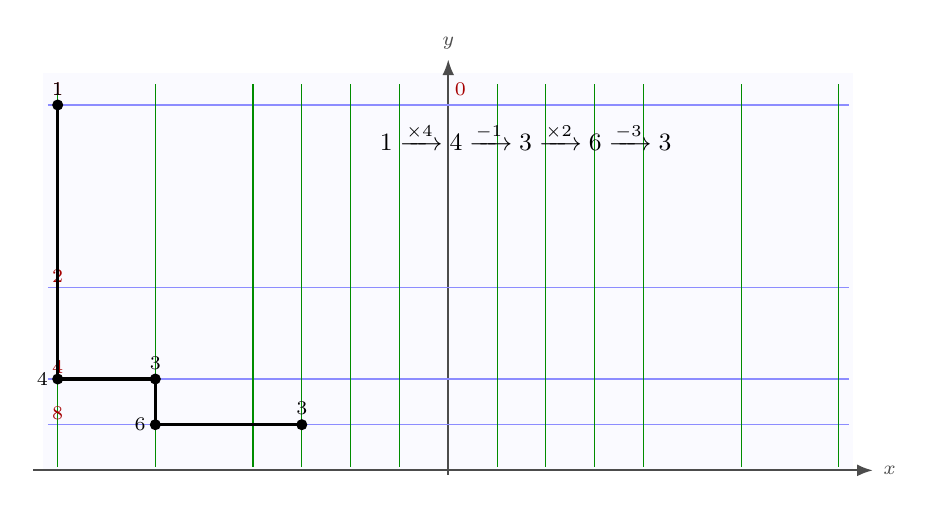
\begin{tikzpicture}[
  x=0.62cm,y=0.58cm,
  axis/.style={-{Latex[length=2mm]},thick,black!70},
  hline/.style={thin,blue!45},
  vline/.style={thin,green!55!black},
  path/.style={very thick,black},
  every node/.style={font=\scriptsize}
]
  \fill[blue!2] (-8.3,0) rectangle (8.3,8.7);
  \draw[axis] (-8.5,0)--(8.7,0) node[right] {$x$};
  \draw[axis] (0,-0.1)--(0,9.0) node[above] {$y$};
  \foreach \yy in {1,2,4,8}
    {\draw[hline] (-8.2,\yy)--(8.2,\yy);}
  \foreach \xx in {-8,-6,-4,-3,-2,-1,1,2,3,4,6,8}
    {\draw[vline] (\xx,0.08)--(\xx,8.45);}
  \node[red!65!black] at (-8.0,8.35) {$1$};
  \node[red!65!black] at (-8.0,4.25) {$2$};
  \node[red!65!black] at (-8.0,2.25) {$4$};
  \node[red!65!black] at (-8.0,1.25) {$8$};
  \node[red!65!black] at (0.25,8.35) {$0$};

  \coordinate (p0) at (-8,8);
  \coordinate (p1) at (-8,2);
  \coordinate (p2) at (-6,2);
  \coordinate (p3) at (-6,1);
  \coordinate (p4) at (-3,1);
  \draw[path] (p0)--(p1)--(p2)--(p3)--(p4);
  \foreach \p/\lab/\pos in {p0/{1}/above,p1/{4}/left,p2/{3}/above,p3/{6}/left,p4/{3}/above}
    {\fill (\p) circle (2pt) node[\pos] {$\lab$};}
  \node[font=\small,anchor=west] at (-1.6,7.3)
    {$1\xrightarrow{\times4}4\xrightarrow{-1}3
      \xrightarrow{\times2}6\xrightarrow{-3}3$};
\end{tikzpicture}
\caption{A schematic point path in the basic hyperbolic arithmetic grid.  The
black polyline retains the intermediate propagation that the endpoint value
forgets.}
\label{fig:p0-path-grid}
\end{figure}

\paragraph{The affine algebra behind the path.}
Every affine prefix has a unique form
\[
  G_i(z)=A_i z+B_i,
  \qquad A_i\ne0.
\]
If $F_i(z)=\alpha_i z+\beta_i$, then
\begin{equation}\label{eq:p0-affine-prefix-recursion}
  A_i=\alpha_i A_{i-1},
  \qquad
  B_i=\alpha_i B_{i-1}+\beta_i,
  \qquad (A_0,B_0)=(1,0).
\end{equation}
The point path is therefore the evaluation of an affine matrix path
\[
  \begin{pmatrix}A_i&B_i\\0&1\end{pmatrix}
  \begin{pmatrix}z_0\\1\end{pmatrix}.
\]
The lower-left entry remains zero at every stage.  Projectively this means that
all prefixes stabilize the same point $\infty$.  Section~\ref{sec:p0-ripples}
shows what changes when right-slot division makes that entry nonzero.

\subsection{Continuous arithmetic motion}
\label{subsec:p0-continuous-motion}

The discrete motions of Subsection~\ref{subsec:p0-point-paths} have an
infinitesimal counterpart.  Translation and dilation generate the Lie algebra
of the positive affine group, and their linear combinations give the continuous
propagation law.  The formulation below is intrinsic: the symbols $u$ and $v$
label arithmetic directions, but need not be coordinates.

\paragraph{The affine Lie algebra and its flow.}
On the assignment line with coordinate $z$, let
\[
 E=\partial_z,
 \qquad
 H=z\partial_z .
\]
These are respectively the infinitesimal generators of translation and positive
dilation, and they satisfy $[E,H]=E$.  Fix constants
$\mu,\lambda\in\mathbb R$, with $\mu\ne0$.  The generator selected by an angle
$\theta$ is
\begin{equation}\label{eq:angular-affine-generator}
 \Omega_\theta
 =\mu\cos\theta\,E+\lambda\sin\theta\,H .
\end{equation}
Consequently, an integral curve $z=z(s)$ satisfies
\begin{equation}\label{eq:continuous-affine-flow}
 \frac{dz}{ds}
 =\mu\cos\theta+\lambda z\sin\theta .
\end{equation}
This Lie-algebra calculation is a derivation of the continuous form of the
arithmetic motion, and it fixes the convention: the translation coefficient is
$\mu\cos\theta$, while the dilation coefficient is $\lambda\sin\theta$.

When $\theta$ is constant, set $b=\lambda\sin\theta$.  The solution through
$z(0)=z_0$ is
\begin{equation}\label{eq:directional-affine-solution}
 z(s)=
 \begin{cases}
  e^{bs}z_0+\displaystyle\mu\cos\theta\,\frac{e^{bs}-1}{b},
     & b\ne0,\\[7pt]
  z_0+\mu s\cos\theta, & b=0.
 \end{cases}
\end{equation}
In particular, the positive arithmetic axes give
\[
 \theta=0:\quad z(s)=z_0+\mu s,
 \qquad
 \theta=\frac{\pi}{2}:\quad z(s)=e^{\lambda s}z_0.
\]
The opposite axes give subtraction and inverse dilation.

\paragraph{The Pfaffian propagation constraint.}
There is a useful three-dimensional local state space with coordinates
$(u,v,z)$.  On it define
\begin{equation}\label{eq:affine-pfaffian-form}
 \alpha=dz-\mu\,du-\lambda z\,dv
\end{equation}
and the two horizontal vector fields
\begin{equation}\label{eq:affine-horizontal-fields}
 D_u=\partial_u+\mu\partial_z,
 \qquad
 D_v=\partial_v+\lambda z\partial_z.
\end{equation}
A curve tangent to
$\cos\theta\,D_u+\sin\theta\,D_v$ satisfies
\eqref{eq:continuous-affine-flow}.  Thus the frequently used notation
\[
 dz=\mu\,du+\lambda z\,dv
\]
means that $\alpha$ vanishes on admissible tangent vectors.  It is not an
identity asserting that $z$ is a function of two independent coordinates whose
ordinary partial derivatives are simultaneously $\mu$ and $\lambda z$.
Indeed,
\begin{equation}\label{eq:horizontal-noncommutation}
 [D_u,D_v]=\mu\lambda\,\partial_z.
\end{equation}
When $\mu\lambda\ne0$, this bracket already rules out such an integrable
coordinate interpretation.  The same bracket is computed intrinsically in
\eqref{eq:arithmetic-frame-bracket-on-a}; the local model here and the frame
there describe one object.  Its geometric reading as a contact structure is
taken up in Section~\ref{sec:p0-contact}.

\begin{theorem}[Continuous affine flow]\label{thm:continuous-affine-flow}
Let $\mathfrak E=(M,g,a;\mu,\lambda)$ be a regular AES with its canonical
arithmetic frame.  If a unit-speed curve $\gamma$ has tangent
\[
 \dot\gamma
 =\cos\theta\,X_u+\sin\theta\,X_v,
\]
where $\theta$ may vary along the curve, then
\begin{equation}\label{eq:intrinsic-continuous-affine-flow}
 \frac{d}{ds}(a\circ\gamma)
 =\mu\cos\theta+\lambda(a\circ\gamma)\sin\theta.
\end{equation}
For constant $\theta$, its solutions are given by \eqref{eq:directional-affine-solution}.
\end{theorem}

\begin{proof}
By the chain rule and \eqref{eq:arithmetic-frame-derivatives},
\[
 \frac{d}{ds}(a\circ\gamma)
 =da(\dot\gamma)
 =\cos\theta\,X_u a+\sin\theta\,X_v a
 =\mu\cos\theta+\lambda a\sin\theta.
\]
For constant $\theta$, this is the linear equation already integrated in
\eqref{eq:directional-affine-solution}.
\end{proof}

\paragraph{Rectification.}
For $\lambda\ne0$, define
\begin{equation}\label{eq:rectifying-assignment}
 r=\operatorname{arcsinh}\!\left(\frac{\lambda a}{\mu}\right).
\end{equation}
The chain rule and \eqref{eq:regular-aes-eikonal} give
\begin{equation}\label{eq:rectified-eikonal}
 |\nabla r|=|\lambda|.
\end{equation}
Thus $r$ has constant gradient magnitude.  When $\lambda=0$, the original
equation already reduces to $|\nabla a|=|\mu|$, and $a/\mu$ is a
unit-gradient rectifying function.  Rectification of the assignment is
possible; rectification of *both* arithmetic directions at once is not, by
\eqref{eq:horizontal-noncommutation}.  This asymmetry is the discrete root of
the tearing language of Section~\ref{sec:p0-holed}.

The same affine convention fixes the sign of the elementary local order defect.
For small increments $h$ and $k$, let
\[
 A_h(z)=z+\mu h,
 \qquad
 M_k(z)=e^{\lambda k}z.
\]
Then
\begin{align}
 (M_k\circ A_h)(z)-(A_h\circ M_k)(z)
 &=\mu h\bigl(e^{\lambda k}-1\bigr)\notag\\
 &=\mu\lambda\,hk+O\!\left(\lVert(h,k)\rVert^3\right).
 \label{eq:infinitesimal-order-defect}
\end{align}
This is an infinitesimal two-order comparison, not an exact area formula for an
arbitrary finite region.  The exact finite statement, and its interpretation as
a defect measured in the commutativized space, occupy
Section~\ref{sec:p0-acs-tearing}.

\paragraph{Affine motion inside projective motion.}
An infinitesimal projective transformation of the line has the Riccati form
\[
 \dot z=\beta+\alpha z+\kappa z^2.
\]
The theory developed in this section is the affine slice $\kappa=0$, with
$\beta=\mu\cos\theta$ and $\alpha=\lambda\sin\theta$.  Results proved for
regular affine AESs do not automatically extend to the quadratic projective
flow.

\subsection{Model names: $E_0$, $E_1$, and later examples}
\label{subsec:p0-model-names}

The historical drafts of this programme used the labels $E_0$ and $E_1$
inconsistently; in some notes the hyperbolic half-plane is called $E_0$, in
others $E_1$.  Because later chapters introduce spaces that are *not* smooth,
we fix the convention now, once, and record it as a convention rather than a
theorem.

\begin{convention}[Model labels]
\label{conv:p0-model-labels}
$\mathfrak E_0(\mu,\lambda)$ denotes the basic regular hyperbolic model of
Subsection~\ref{subsec:p0-basic-model}.  For $k\ge1$, the label
$\mathfrak E_k$ is used descriptively for an arithmetic expression space whose
regular locus is a surface with $k$ declared punctures: points removed from the
regular structure and carrying no regular AES data.  No classification by $k$
is asserted; the label records the number of declared punctures and nothing
else.  The reserved historical labels $E_k$ and $E_{\log}$ of earlier drafts
are not model classes, and this paper defines neither of them.
\end{convention}

Two examples make the convention concrete; both are developed later, and the
first one is the only example in this paper whose punctured model is verified
in detail.

\begin{example}[The basic model, $k=0$]
\label{ex:p0-e0-model}
$\mathfrak E_0(\mu,\lambda)$ is the upper half-plane with the metric
\eqref{eq:p0-e0-data} and the assignment $a=-x/y$.  It has no puncture, its
assignment vanishes along one complete geodesic, and by
Theorem~\ref{thm:basic-hyperbolic-aes} it is complete with constant curvature.
This is the model in which the arithmetic motions of
Subsection~\ref{subsec:p0-point-paths} are read as point paths.
\end{example}

\begin{example}[A one-puncture model, $k=1$]
\label{ex:p0-e1-model}
Let $\mathbb D=\{\rho<1\}$ be the unit disc with the complete Poincar\'e
metric $g_{\mathbb D}=4\,(d\xi^2+d\eta^2)/\lambda^2(1-\rho^2)^2$ and the radial
assignment
\[
 a_{\mathbb D}(\xi,\eta)=
 \begin{cases}
  \dfrac{2\mu}{\lambda}\,\dfrac{\rho}{1-\rho^2},&\rho\ne0,\\[6pt]
  0,&\rho=0 .
 \end{cases}
\]
On the punctured disc $\mathbb D\setminus\{0\}$ this is a regular AES with
$|\nabla a_{\mathbb D}|^2=\mu^2+\lambda^2a_{\mathbb D}^2$, while at the centre
the assignment fails to be $C^1$ although the metric extends smoothly.  The
regular locus is therefore $\mathbb D\setminus\{0\}$ and the model carries
exactly one puncture.  Paper~I verifies the details of this model as its
isolated-zero example; the global invariant $\lambda a_{\mathbb D}
=\mu\sinh(\lambda s)$ along hyperbolic distance $s$ from the centre shows that
the assignment, not the metric, is what fails at the puncture.
\end{example}

Example~\ref{ex:p0-e1-model} is the first holed arithmetic expression space, and
Section~\ref{sec:p0-holed} returns to it.  Its puncture is not a hole in the
metric; it is a point at which the regular structure stops being defined, and
it is where the arithmetic motions of the punctured part can no longer be
extended.


\section{Ripple Geometry: The Projective Dual}\label{sec:p0-ripples}
A point path follows one chosen input through a sequence of motions.  The
projective operation $c/z$ admits no such motion of the value, and the
observation of Subsection~\ref{subsec:p0-point-paths} was that its matrix has a
nonzero lower-left entry.  There is nevertheless a geometry attached to it, and
it is obtained by reversing the direction of the reading: instead of pushing a
point forward, pull an entire output condition backward through the same maps.
The upper half-plane makes this dual reading elementary, because M\"obius maps
carry generalized circles to generalized circles.

We call the resulting picture \emph{ripple geometry}: the family of conditions
obtained by pulling output conditions back through a projective arithmetic
operator.  The name is descriptive, and
Subsection~\ref{subsec:p0-ripple-status} states precisely what it does and does
not assert.

\subsection{Poles and standard horocycles}

Let
\begin{equation}\label{eq:p0-mobius-map}
  F(z)=\frac{Az+B}{Cz+D}
\end{equation}
be a real fractional linear map with
\[
  \Delta=AD-BC>0.
\]
The positivity convention ensures that $F$ maps the upper half-plane to itself.
The projective pole is
\[
  p_F=F^{-1}(\infty)
  =\begin{cases}
     -D/C,&C\ne0,\\
     \infty,&C=0.
   \end{cases}
\]
For $t>0$, denote the standard horocycle based at infinity by
\[
  \mathcal H_t=\{w\in\mathbb H:\im w=t\}.
\]

\begin{definition}[Ripple pencil]
\label{def:p0-ripple-pencil}
The \emph{ripple pencil} of $F$ is the one-parameter family
\[
  \mathcal R(F)
  =\{F^{-1}(\mathcal H_t):t>0\}.
\]
It is a family of horocycles based at the pole $p_F$.  The word ``ripple'' is a
visual name for this standard M\"obius pullback family.
\end{definition}

\begin{theorem}[Line-to-circle transition]
\label{thm:p0-ripple-pencil-formula}
Let $F$ be as in \eqref{eq:p0-mobius-map}.

\begin{enumerate}
  \item If $C=0$, every member of $\mathcal R(F)$ is a horizontal line; the
  pencil is based at $\infty$.

  \item If $C\ne0$, the member with parameter $t$ is the Euclidean circle
  \begin{equation}\label{eq:p0-ripple-circle}
    \left(x+\frac DC\right)^2
    +\left(y-\frac{\Delta}{2tC^2}\right)^2
    =\left(\frac{\Delta}{2tC^2}\right)^2.
  \end{equation}
  All these circles are tangent to the real boundary at the common point
  $p_F=-D/C$ and are nested as $t$ varies.
\end{enumerate}
\end{theorem}

\begin{proof}
For $z=x+iy$, direct calculation gives the standard identity
\begin{equation}\label{eq:p0-imaginary-mobius}
  \im F(z)=\frac{\Delta y}{|Cz+D|^2}.
\end{equation}
The inverse image of $\mathcal H_t$ is therefore
\[
  \Delta y=t\bigl((Cx+D)^2+C^2y^2\bigr).
\]
If $C=0$, this reduces to a horizontal line.  If $C\ne0$, divide by
$tC^2$ and complete the square in $y$:
\[
  \left(x+\frac DC\right)^2+y^2
  -\frac{\Delta}{tC^2}y=0,
\]
which is exactly \eqref{eq:p0-ripple-circle}.  The center lies vertically
above $-D/C$ at a height equal to the radius, so the circle is tangent to the
boundary there.  The radius is proportional to $t^{-1}$, proving nesting.
\end{proof}

The theorem gives a geometric interpretation of the lower-left matrix entry.
The affine condition $C=0$ places the pole at infinity and degenerates the
ripple circles to parallel lines.  A projective step with $C\ne0$ moves the pole
to a finite boundary point and curves the same horocyclic family into visible
ripples.

\begin{example}[Arithmetic inversion]
\label{ex:p0-inversion-ripples}
For
\[
  J(z)=-\frac1z,
  \qquad
  J\leftrightarrow
  \begin{pmatrix}0&-1\\1&0\end{pmatrix},
\]
one has $p_J=0$ and
\begin{equation}\label{eq:p0-inversion-circles}
  x^2+\left(y-\frac1{2t}\right)^2
  =\left(\frac1{2t}\right)^2.
\end{equation}
Thus inversion turns the horizontal horocycles based at infinity into a nested
family of circles tangent at zero.  The map exchanges the two ideal points
$0$ and $\infty$.
\end{example}

\begin{figure}[t]
\centering
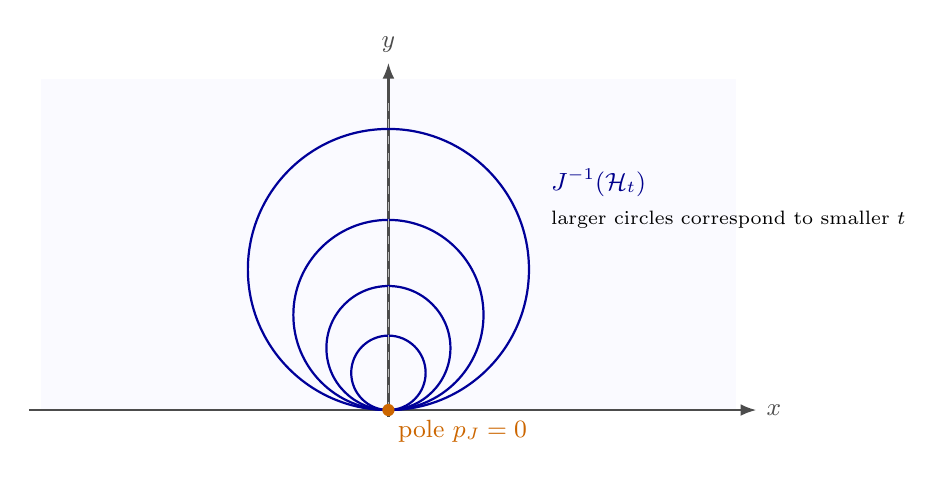
\begin{tikzpicture}[
  x=1.05cm,y=1.05cm,
  axis/.style={-{Latex[length=2mm]},thick,black!70},
  ripple/.style={thick,blue!60!black},
  geod/.style={dashed,gray!55},
  every node/.style={font=\small}
]
  \fill[blue!2] (-4.2,0) rectangle (4.2,4.0);
  \draw[axis] (-4.35,0)--(4.45,0) node[right] {$x$};
  \draw[axis] (0,-0.08)--(0,4.2) node[above] {$y$};
  \foreach \r in {0.45,0.75,1.15,1.7}
    {\draw[ripple] (0,\r) circle (\r);}
  \draw[geod] (0,0)--(0,3.75);
  \fill[orange!80!black] (0,0) circle (2.2pt)
    node[below right] {pole $p_J=0$};
  \node[blue!55!black,anchor=west] at (1.85,2.75)
    {$J^{-1}(\mathcal H_t)$};
  \node[anchor=west,font=\scriptsize] at (1.85,2.3)
    {larger circles correspond to smaller $t$};
\end{tikzpicture}
\caption{The ripple pencil of inversion.  Every circle is a horocycle tangent
at the projective pole $0$; the affine horizontal-line pencil is recovered
when the pole is moved to infinity.}
\label{fig:p0-inversion-ripple-pencil}
\end{figure}

\begin{remark}[Which upper half-plane, and with which metric]
\label{rem:p0-ripple-normalization}
The complex coordinate used throughout this section is the Möbius continuation
chart, and it is not literally the point coordinate of
Section~\ref{sec:p0-aes}.  With the metric $g_{\mu,\lambda}$ of
\eqref{eq:p0-e0-data}, the chart in which the horocycles are the Euclidean
horizontal lines and the metric is the standard one of curvature $-1$ is
\[
  Z=\frac{\lambda}{\mu}x+iy,
\]
as follows from \eqref{eq:scaled-standard-hyperbolic-metric}.  When
$\mu=\lambda$ this is the identity, which is why the two roles of $x+iy$ are
usually identified in the literature; here they are kept apart, and all
Möbius statements below are made in the $Z$-chart.  Only when a statement
concerns the assignment $a$ rather than the metric do we return to $(x,y)$.
\end{remark}

\subsection{Zero--pole pencils in the complex chart}

There is a second elementary pencil attached to the same operator.  Suppose
$A,C\ne0$ and write its zero and pole as
\[
  q_F=-\frac BA,
  \qquad
  p_F=-\frac DC.
\]
Then the output level set $|F(z)|=r$ is equivalent to
\begin{equation}\label{eq:p0-apollonius-pencil}
  |z-q_F|
  =r\left|\frac CA\right|\,|z-p_F|.
\end{equation}
For $r|C/A|\ne1$ these are Apollonius circles; for $r|C/A|=1$ the locus is the
perpendicular bisector line of the segment $q_Fp_F$, that is, a generalized
circle of infinite radius.  The horocyclic
ripple pencil and the Apollonius pencil encode different output observables,
$\im F$ and $|F|$, but both show that a projective one-hole operator naturally
carries more than a point orbit: it carries a zero, a pole, and a family of
generalized circles organized by them.

\subsection{Ripple histories of right-expanded expressions}

Let a right-expanded expression determine nondegenerate real M\"obius sections
$F_1,\ldots,F_n$ of \emph{positive} determinant, in chronological order, and
write
\[
  G_k=F_k\circ\cdots\circ F_1,
  \qquad
  G_k(z)=\frac{A_kz+B_k}{C_kz+D_k}.
\]
At stage $k$, the arithmetic value of a chosen input follows the point orbit
$G_k(z_0)$.  Simultaneously, the output horocycles pull back to
\[
  \mathcal R_k=\mathcal R(G_k).
\]
The tangency point
\[
  p_k=G_k^{-1}(\infty)
  =-\frac{D_k}{C_k}
\]
when $C_k\ne0$ is the current pole of the prefix operator.

Thus a general right-expansion history should not be pictured as one fixed
family of concentric circles.  Each prefix has its own ripple pencil, and the
common tangency point of that pencil may move with $k$.  The appropriate
geometric state is
\[
  \bigl(G_k,\,G_k(z_0),\,p_k,\,\mathcal R_k\bigr):
\]
the operator, the selected point, the pole, and the pulled-back wavefront
family.

\begin{proposition}[Covariant--contravariant duality]
\label{prop:p0-path-ripple-duality}
For every prefix operator $G_k$ and every output horocycle $\mathcal H_t$,
\[
  z_0\in G_k^{-1}(\mathcal H_t)
  \quad\Longleftrightarrow\quad
  G_k(z_0)\in\mathcal H_t.
\]
Hence the point path and the ripple history are two readings of the same
operator word: one pushes the input forward, the other pulls the output
condition backward.
\end{proposition}

\begin{proof}
This is the defining property of inverse image.
\end{proof}

The elementary nature of the proposition is precisely its value.  No new
geometry is inserted between the two pictures.  Their unity is already present
in the action of one M\"obius matrix.

\subsection{The status of ripple geometry}
\label{subsec:p0-ripple-status}

The preceding constructions are elementary and proved.  The name
``ripple geometry'' is not, and it is important to separate the two.

\begin{itemize}
  \item \emph{What is proved.}  A real orientation-preserving M\"obius map
  pulls the standard horocycle $\mathcal H_t$ back to a line (when its pole is
  infinity) or to a circle tangent to the boundary at its pole, and these
  circles are nested; the pole is the inverse image of infinity; the same
  prefix matrix determines the point orbit, the pole, the fixed points, and the
  ripple pencil.
  \item \emph{What is descriptive.}  ``Ripple geometry'' names the dual reading
  in which the operator acts on conditions instead of points.  It does not
  assert a new isomorphism class of hyperbolic or projective geometry, a new
  invariant of arithmetic words, or the existence of a projective arithmetic
  expression space.
  \item \emph{What is open.}  Whether the ripple family, taken together with
  its moving pole, is intrinsic to the arithmetic word rather than to a chosen
  upper-half-plane chart; which path or ripple data descend through relations
  among history words; and whether a punctured model in the sense of
  Section~\ref{sec:p0-holed} carries a ripple structure that survives at the
  puncture.
\end{itemize}

The reason for keeping the name is that the dual reading is what makes
division homogeneous with the other operations at the level of *conditions*:
addition, subtraction, and multiplication by a constant move the value and
hence move the contours of the assignment, while second-slot division moves the
contours without moving the value affinely.  The reason for keeping it
provisional is that no intrinsic formulation of that observation is available
yet; the current statement of it depends on the standard horocycle
$\mathcal H_t$ and therefore on one chart.


\section{Reciprocals, Poles, Infinity, and Fixed Points}\label{sec:p0-reciprocals}
Right-slot division makes three elementary notions meet: reciprocal
arithmetic, a pole in an affine chart, and the projective point at infinity.
Iteration adds a fourth notion: a finite or infinite expression can be the
closure of a recurrence at one of its fixed points.  This section keeps the
algebraic fixed-point equation, analytic convergence, and projective
continuation distinct.

\subsection{Arithmetic reciprocals and projective poles}

For $c\ne0$, the ordinary map
\[
  J_c(z)=\frac{c}{z}
\]
is defined on $K\setminus\{0\}$.  Its projective matrix is
\[
  J_c\leftrightarrow
  \begin{pmatrix}0&c\\1&0\end{pmatrix},
\]
so on $\PP^1(K)$ it satisfies
\[
  J_c(0)=\infty,
  \qquad
  J_c(\infty)=0.
\]
The projective statements do not make ordinary division by zero admissible;
they record the chart transition of the associated fractional linear map.

More generally, the reciprocal coordinate centered at a finite point $q$ is
\begin{equation}\label{eq:p0-pole-coordinate}
  w_q(z)=\frac1{z-q}.
\end{equation}
It sends $q$ to infinity and infinity to zero.  In this coordinate, rational
functions with no finite pole except possibly $q$ become polynomials in
$w_q$:
\[
  K[w_q]=K\!\left[\frac1{z-q}\right].
\]
The usual polynomial chart $K[z]$ is the corresponding chart whose distinguished
pole is $\infty$.  This is an elementary coordinate observation, not a claim
that one pole chart is globally preferable to another.

\begin{remark}[The pole as a ripple center]
By Theorem~\ref{thm:p0-ripple-pencil-formula}, the same point $q$ that is sent
to infinity by $w_q$ is the common boundary tangency point of the pulled-back
horocycles.  Thus the algebraic denominator zero and the geometric ripple
center are two readings of the same projective datum.
\end{remark}

\subsection{A reciprocal as the closure of an infinite expansion}

Consider a scalar parameter $r$ and the affine recursion
\begin{equation}\label{eq:p0-geometric-recursion}
  S_0=0,
  \qquad
  S_{n+1}=1+rS_n.
\end{equation}
The first terms are
\[
  0,\quad 1,\quad 1+r,\quad 1+r+r^2,\quad\ldots.
\]
As a nested right-expanded expression,
\[
  S_n=1+r\bigl(1+r(\cdots(1+r\cdot0)\cdots)\bigr).
\]
Since scalar multiplication is commutative, this example does not by itself
distinguish left and right placement; its role is to show how an arithmetic
reciprocal arises from recursive closure.

\begin{proposition}[Finite geometric expansion]
\label{prop:p0-finite-geometric-expansion}
For every $n\ge0$,
\[
  S_n=\sum_{k=0}^{n-1}r^k.
\]
If $r\ne1$, then
\begin{equation}\label{eq:p0-finite-geometric-quotient}
  S_n=\frac{1-r^n}{1-r}.
\end{equation}
If $K=\R$ or $\C$ and $|r|<1$, then
\[
  S_n\longrightarrow\frac1{1-r}.
\]
The same identity holds formally in $K[[r]]$ as
$(1-r)^{-1}=\sum_{k\ge0}r^k$.
\end{proposition}

\begin{proof}
Induction in \eqref{eq:p0-geometric-recursion} gives the finite sum.  Multiplying
that sum by $1-r$ telescopes to $1-r^n$, proving
\eqref{eq:p0-finite-geometric-quotient}.  Under $|r|<1$, one has $r^n\to0$.
The formal-power-series statement follows because multiplication by $1-r$
leaves the constant series $1$ coefficient by coefficient.
\end{proof}

The convergence hypothesis is active.  For example, $r=-1$ makes the sequence
oscillate, and $|r|>1$ generally makes its finite values grow rather than
converge.  The algebraic reciprocal $1/(1-r)$ may exist even when the forward
iteration does not converge to it.

\subsection{Fixed-point closure and escape to infinity}

Let
\[
  T_r(s)=1+rs.
\]
A finite fixed point satisfies
\[
  s=T_r(s)
  \quad\Longleftrightarrow\quad
  (1-r)s=1.
\]
Hence
\begin{equation}\label{eq:p0-geometric-fixed-point}
  q_r=\frac1{1-r}
\end{equation}
when $r\ne1$.  The geometric series therefore converges, when $|r|<1$, to the
finite fixed point of the update that generates its truncations.

The projective matrix of $T_r$ is
\[
  M_r=
  \begin{pmatrix}r&1\\0&1\end{pmatrix}.
\]
It always fixes $\infty$.  If $r\ne1$, it has the second fixed point $q_r$.
As $r\to1$, the finite point $q_r$ leaves every compact subset of the affine
line and approaches $\infty$ in $\PP^1$.  At $r=1$ the update becomes the
translation
\[
  T_1(s)=s+1,
\]
which has no finite fixed point and has $\infty$ as its repeated projective
fixed point.  Thus the pole of the parameter function $r\mapsto1/(1-r)$ is
exactly the parameter at which finite fixed-point closure degenerates into a
parabolic fixed point at infinity.

The same mechanism holds for a general invertible affine map.

\begin{proposition}[Affine iteration and its fixed point]
\label{prop:p0-affine-iteration}
Let
\[
  T(z)=az+b,
  \qquad a\ne0.
\]
If $a\ne1$, put
\[
  q=\frac{b}{1-a}.
\]
Then
\begin{equation}\label{eq:p0-affine-centered-form}
  T(z)=q+a(z-q),
  \qquad
  T^n(z)=q+a^n(z-q).
\end{equation}
Consequently, over $\R$ or $\C$, $T^n(z)\to q$ for every finite $z$ when
$|a|<1$.  If $a=1$ and $b\ne0$, the only projective fixed point is
$\infty$ and $T^n(z)=z+nb$.
\end{proposition}

\begin{proof}
The equation $(1-a)q=b$ gives the centered form.  Iteration of that form gives
\eqref{eq:p0-affine-centered-form} by induction.  The convergence and
translation statements are immediate.
\end{proof}

This proposition separates three notions:

\begin{itemize}
  \item the algebraic existence of a finite fixed point;
  \item attraction of an orbit to that point;
  \item the projective fixed point at infinity already carried by every affine
  operator.
\end{itemize}

They coincide only under additional hypotheses.

\subsection{Right reciprocal iteration and continued fractions}

A stationary right-expanded reciprocal update has the form
\begin{equation}\label{eq:p0-right-reciprocal-map}
  F(z)=a+\frac{b}{z},
  \qquad b\ne0,
\end{equation}
with projective matrix
\[
  M_F=
  \begin{pmatrix}a&b\\1&0\end{pmatrix}.
\]
The ordinary iteration is defined only while no intermediate denominator
vanishes.  Its finite truncations are generalized continued fractions:
\[
  z_n
  =a+\cfrac{b}{a+\cfrac{b}{\ddots+\cfrac{b}{z_0}}}.
\]
The matrix formulation remains projectively meaningful when an affine
intermediate value passes through infinity.

\begin{proposition}[Fixed points of a reciprocal update]
\label{prop:p0-reciprocal-fixed-points}
The finite fixed points of \eqref{eq:p0-right-reciprocal-map} are the roots of
\begin{equation}\label{eq:p0-reciprocal-quadratic}
  z^2-az-b=0.
\end{equation}
At a nonzero fixed point $q$,
\[
  F'(q)=-\frac{b}{q^2}.
\]
Over $\C$, if $|F'(q)|<1$, then $q$ is locally attracting; if
$|F'(q)|>1$, it is locally repelling.
\end{proposition}

\begin{proof}
Multiplying $q=a+b/q$ by $q$ gives
\eqref{eq:p0-reciprocal-quadratic}.  Differentiation gives the multiplier.
The local dynamical classification is the standard contraction/expansion test
from the first nonzero derivative.
\end{proof}

\begin{example}[The golden-ratio expansion]
\label{ex:p0-golden-ratio}
Take
\[
  F(z)=1+\frac1z,
  \qquad z_0=1.
\]
Then
\[
  1,\quad2,\quad\frac32,\quad\frac53,\quad\frac85,\ldots
\]
are ratios of consecutive Fibonacci numbers.  The fixed points solve
\[
  z^2-z-1=0,
\]
so they are
\[
  \phi=\frac{1+\sqrt5}{2},
  \qquad
  -\phi^{-1}=\frac{1-\sqrt5}{2}.
\]
Since $|F'(\phi)|=\phi^{-2}<1$, the positive fixed point is attracting for
nearby positive initial values.  The infinite continued fraction
\[
  1+\cfrac1{1+\cfrac1{1+\cdots}}
\]
therefore denotes $\phi$ only after the convergence statement has been
established; the fixed-point equation alone does not choose the attracting
root in every field or domain.
\end{example}

For nonstationary data,
\[
  F_k(z)=a_k+\frac{b_k}{z},
  \qquad
  M_k=\begin{pmatrix}a_k&b_k\\1&0\end{pmatrix},
\]
and the $n$th truncation is represented by the product
\[
  M_nM_{n-1}\cdots M_1.
\]
This is the first place where the nested visual form, the ordinary recurrence,
and matrix multiplication become exactly the same calculation.

\subsection{Fixed points of a general projective operator}

Let
\[
  F(z)=\frac{Az+B}{Cz+D},
  \qquad \Delta=AD-BC\ne0.
\]
A finite fixed point satisfies
\begin{equation}\label{eq:p0-general-mobius-fixed-point}
  Cz^2+(D-A)z-B=0.
\end{equation}
In homogeneous coordinates, fixed points are precisely the eigenlines of the
matrix
\[
  \begin{pmatrix}A&B\\C&D\end{pmatrix}.
\]
The point $\infty$ is fixed exactly when $C=0$.  Over an algebraic closure a
nonidentity projective map has two fixed points counted with multiplicity; over
the base field those points may be distinct, repeated, or visible only after a
field extension.

This completes the elementary circle of ideas:
\[
  \text{reciprocal}
  \longrightarrow
  \text{pole}
  \longrightarrow
  \infty
  \longrightarrow
  \text{fixed-point closure}
  \longrightarrow
  \text{matrix eigenline}.
\]
The next section shows that the same matrix also governs point paths and ripple
pencils.


\section{Matrix and Projective Unification}\label{sec:p0-projective-unification}
The two geometric pictures now have a common algebraic carrier.  A one-hole
arithmetic section is represented by a $2\times2$ matrix; chronological
composition is matrix multiplication, point paths are matrix orbits, ripple
pencils are inverse images under the same products, poles are inverse images
of infinity, and fixed points are eigenlines.

\subsection{Elementary arithmetic matrices}

Let $K$ be a field.  In homogeneous coordinates, write
\[
  z=[z:1],
  \qquad
  \infty=[1:0],
\]
and let
\[
  M=\begin{pmatrix}A&B\\C&D\end{pmatrix}
\]
act by
\[
  M\cdot z=\frac{Az+B}{Cz+D}.
\]
Nonzero scalar multiples represent the same element of $\PGL_2(K)$.

The nondegenerate elementary sections have the following representatives.

\begin{center}
\renewcommand{\arraystretch}{1.4}
\begin{tabular}{lll}
\toprule
one-hole section & affine formula & matrix \\
\midrule
$C^{(1)}_{+,c}=C^{(2)}_{+,c}$
& $z+c$
& $\begin{pmatrix}1&c\\0&1\end{pmatrix}$ \\
$C^{(1)}_{-,c}$
& $z-c$
& $\begin{pmatrix}1&-c\\0&1\end{pmatrix}$ \\
$C^{(2)}_{-,c}$
& $c-z$
& $\begin{pmatrix}-1&c\\0&1\end{pmatrix}$ \\
$C^{(1)}_{\times,c}=C^{(2)}_{\times,c}$
& $cz$
& $\begin{pmatrix}c&0\\0&1\end{pmatrix}$ \\
$C^{(1)}_{/,c}$
& $z/c$
& $\begin{pmatrix}1&0\\0&c\end{pmatrix}$ \\
$C^{(2)}_{/,c}$
& $c/z$
& $\begin{pmatrix}0&c\\1&0\end{pmatrix}$ \\
\bottomrule
\end{tabular}
\end{center}

Here $c\ne0$ whenever invertibility requires it.  The table has two immediate
consequences.

\begin{enumerate}
  \item Every pure slot-$(1)$ section is affine and fixes $\infty$.
  \item The projectively new primitive is slot-$(2)$ division.  Up to a
  nonzero scaling, it is inversion.
\end{enumerate}

Ordinary arithmetic and projective continuation remain separate.  A matrix in
$\PGL_2(K)$ acts everywhere on $\PP^1(K)$, while the corresponding ordinary
word may be undefined at an intermediate denominator zero.

\subsection{Chronological products}

Let $F_1,\ldots,F_n$ be nondegenerate sections with matrix representatives
$M_1,\ldots,M_n$, and suppose $F_1$ is applied first.  Define
\begin{equation}\label{eq:p0-prefix-matrices}
  P_k=M_kM_{k-1}\cdots M_1,
  \qquad
  G_k=F_k\circ\cdots\circ F_1.
\end{equation}
Then $P_k$ represents $G_k$.

\begin{theorem}[One matrix, four readings]
\label{thm:p0-four-matrix-readings}
Write
\[
  P_k=\begin{pmatrix}A_k&B_k\\C_k&D_k\end{pmatrix}.
\]
The same prefix matrix determines:

\begin{enumerate}
  \item the point-path state
  \[
    z_k=G_k(z_0)=\frac{A_kz_0+B_k}{C_kz_0+D_k};
  \]

  \item the projective pole
  \[
    p_k=G_k^{-1}(\infty)
      =-D_k/C_k
  \]
  when $C_k\ne0$, and $p_k=\infty$ when $C_k=0$;

  \item the fixed-point equation
  \[
    C_kz^2+(D_k-A_k)z-B_k=0;
  \]

  \item over $\R$, when a lift has positive determinant, the ripple pencil
  $G_k^{-1}(\mathcal H_t)$ from
  Theorem~\ref{thm:p0-ripple-pencil-formula}.
\end{enumerate}
\end{theorem}

\begin{proof}
The first formula is the matrix action.  The pole solves
$C_kz+D_k=0$.  The fixed-point equation comes from
$z(C_kz+D_k)=A_kz+B_k$.  The final statement is the definition of the ripple
pencil together with formula \eqref{eq:p0-imaginary-mobius}.
\end{proof}

Thus \emph{path} and \emph{ripple} are not two unrelated representations.  They
are the covariant and contravariant geometries of one chronological matrix
product.

\begin{figure}[t]
\centering
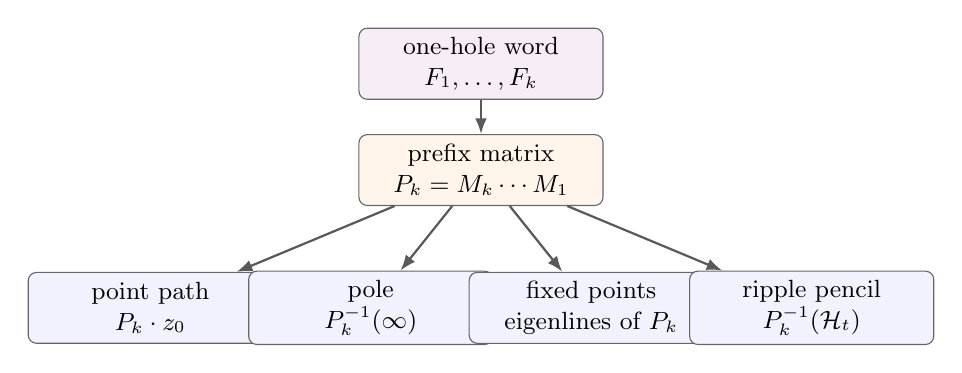
\begin{tikzpicture}[
  box/.style={draw=black!60,rounded corners=3pt,fill=blue!5,
              minimum width=31mm,minimum height=9mm,align=center,font=\small},
  arr/.style={-{Latex[length=2mm]},thick,black!65},
  every node/.style={font=\small}
]
  \node[box,fill=violet!7] (word) at (0,2.0)
    {one-hole word\\$F_1,\ldots,F_k$};
  \node[box,fill=orange!8] (matrix) at (0,0.65)
    {prefix matrix\\$P_k=M_k\cdots M_1$};
  \node[box] (path) at (-4.2,-1.1) {point path\\$P_k\cdot z_0$};
  \node[box] (pole) at (-1.4,-1.1) {pole\\$P_k^{-1}(\infty)$};
  \node[box] (fixed) at (1.4,-1.1) {fixed points\\eigenlines of $P_k$};
  \node[box] (ripple) at (4.2,-1.1) {ripple pencil\\$P_k^{-1}(\mathcal H_t)$};
  \draw[arr] (word)--(matrix);
  \foreach \n in {path,pole,fixed,ripple}
    {\draw[arr] (matrix)--(\n);}
\end{tikzpicture}
\caption{Four geometric readings of the same chronological matrix product.}
\label{fig:p0-projective-four-readings}
\end{figure}

\subsection{The affine chart as the stabilizer of infinity}

Let
\[
  B_\infty=\Stab_{\PGL_2(K)}(\infty).
\]
A matrix fixes infinity exactly when $C=0$.  After projective rescaling, every
such element has a unique representative
\[
  \begin{pmatrix}a&b\\0&1\end{pmatrix},
  \qquad a\in K^\times,\quad b\in K,
\]
and acts as $z\mapsto az+b$.  Hence
\begin{equation}\label{eq:p0-affine-stabilizer}
  B_\infty\cong\Aff(1,K).
\end{equation}

This identifies the path geometry of Section~\ref{sec:p0-paths} as a
pole-at-infinity gauge.  In that gauge:

\begin{itemize}
  \item the denominator is constant;
  \item the ripple pencil is a parallel-line pencil;
  \item fixed-point recursion is affine;
  \item the lower-left matrix entry stays zero.
\end{itemize}

Choosing a finite pole $q$ amounts to conjugating this affine subgroup by a
projective map sending $q$ to infinity.  The coordinate
$w_q=1/(z-q)$ from \eqref{eq:p0-pole-coordinate} is the simplest such gauge.

\subsection{Generation of the projective group}

Introduce
\[
  T_s(z)=z+s,
  \qquad
  D_q(z)=qz\quad(q\ne0),
  \qquad
  J(z)=-\frac1z.
\]
They arise respectively from addition, multiplication, and second-slot
division.

\begin{theorem}[Elementary projective generation]
\label{thm:p0-pgl2-generation}
For every field $K$, translations $T_s$, nonzero scalings $D_q$, and inversion
$J$ generate $\PGL_2(K)$.  Equivalently, the projective evaluations of
nondegenerate left- and right-slot arithmetic sections have image
$\PGL_2(K)$.
\end{theorem}

\begin{proof}
Let
\[
  F(z)=\frac{Az+B}{Cz+D},
  \qquad AD-BC\ne0.
\]
If $C=0$, then $A,D\ne0$ and
\[
  F=T_{B/D}\circ D_{A/D}.
\]
If $C\ne0$, direct calculation gives
\begin{equation}\label{eq:p0-projective-factorization}
  F
  =T_{A/C}
   \circ D_{(AD-BC)/C^2}
   \circ J
   \circ T_{D/C}.
\end{equation}
All scale parameters are nonzero, so every factor is available.  These two
cases exhaust $\PGL_2(K)$.
\end{proof}

The proof also yields the rank-one Bruhat decomposition
\begin{equation}\label{eq:p0-bruhat}
  \PGL_2(K)=B_\infty\sqcup B_\infty J B_\infty.
\end{equation}
The first cell consists of operators whose pole is infinity.  The second
consists of operators with a finite pole in the chosen affine chart.  Thus the
transition from a point-path grid to a curved ripple pencil is the elementary
geometric face of crossing from the affine cell to the projective cell.

\subsection{Left and right representations in one projective plane}

We can now answer the algebraic comparison of the two combs precisely.

\begin{theorem}[Projective unification of the two combs]
\label{thm:p0-comb-projective-unification}
The left- and right-expanded combs have the same abstract chain of internal
dependencies and are exchanged by the opposite-operation involution of
Proposition~\ref{prop:p0-comb-opposition}.  Their one-hole operator images have
the following relation:

\begin{enumerate}
  \item the pure left-expanded nondegenerate language lies in
  $B_\infty\cong\Aff(1,K)$;

  \item the pure right-expanded language already contains translations,
  nonzero scalings, reflections, and inversion, and therefore generates
  $\PGL_2(K)$;

  \item after embedding both languages into $\PGL_2(K)$, their point paths,
  poles, fixed points, and ripple pencils are all read from the same matrix
  representation.
\end{enumerate}
\end{theorem}

\begin{proof}
The dependency and opposition statements were proved in
Section~\ref{sec:p0-two-combs}.  The elementary table shows that every
slot-$(1)$ generator fixes infinity.  The pure slot-$(2)$ language contains
$T_s$ because addition is commutative, contains $D_q$ because multiplication
is commutative, and contains $J$ through second-slot division.  Apply
Theorem~\ref{thm:p0-pgl2-generation}.  The last assertion is
Theorem~\ref{thm:p0-four-matrix-readings}.
\end{proof}

The theorem does not say that a left-expanded word and a right-expanded word
with the same constants have the same operator.  It says that their apparently
different elementary geometries live in one projective action and can be
compared there without erasing operand-slot information.


\section{Affine Cocycles and the Relative Defect}\label{sec:p0-affine-cocycles}
\input{sections/07-affine-cocycles.tex}

\section{Commutativization: The ACS and Arithmetic Tearing}\label{sec:p0-acs-tearing}
% Moved from Paper I Section 8 (governance/00b, migration map); mathematical content
% unchanged apart from cross-references, framing sentences, and the closing
% subsection on tearing.
The arithmetic motions of Section~\ref{sec:p0-aes} do not commute: addition and
multiplication transport each other's rulers by the Baumslag--Solitar-type
relation \eqref{eq:p0-bs-relation}, and the affine cocycle of
Section~\ref{sec:p0-affine-cocycles} records the resulting order dependence in
two translation coordinates.  This section constructs a commutativization of
that non-commutative motion, and the level at which commutation is imposed must
be stated exactly.

Take the history language itself: the free monoid generated by the two families
of one-step histories, additive steps and multiplicative steps.  Impose that
generators of the two families commute.  Equivalently --- and this is the form
used below --- keep the total additive charge and the total logarithmic
multiplicative charge of a history and forget the order in which they were
accumulated; the charges satisfy the imposed commutation by construction.  The
resulting object is a plane with two coordinates, and we call it the
\emph{accumulative commutative space}, ACS.  The construction has two distinct
uses, and they must not be conflated.  For a positive add--scale history it
records the two total charges; and it supplies a weighted integral along the
charge path whose value restores the
translation part that the charge endpoint alone forgets.  The ACS is therefore a
*shadow* of
the presented history: it is a commutative quotient object attached to a
non-commutative one, not another presentation of the full arithmetic syntax.

This is *not* the abelianization of the group of affine motions, and the
difference is worth recording once.  In $\operatorname{Aff}^{+}(1,\mathbb R)$
one has $D_kT_pD_k^{-1}T_p^{-1}=T_{(k-1)p}$, so the commutator subgroup is the
translation subgroup and the abelianization keeps the scale alone:
\[
  \operatorname{Aff}^{+}(1,\mathbb R)_{\mathrm{ab}}
  \;\cong\;\mathbb R_{>0}\;\cong\;(\mathbb R,+).
\]
The ACS keeps the additive charge as well, because it is attached to the
presented histories *before* evaluation rather than to their images in the
affine group.  The hierarchy --- literal histories, then charges, then evaluated
motions --- is accordingly not a convenience of exposition; collapsing it
changes the object.  Subsection~\ref{subsec:p0-acs-forgets} states what the ACS
forgets, and the distributivity example of
Subsection~\ref{subsec:p0-distributivity} already shows why the charge map
cannot be pushed through the operator quotient.

The geometric use is the reason for the name of this chapter.  Two histories
with the same charge endpoint have charge paths that
together bound a region of the ACS, and the exact value of their order defect is
a weighted area of that region (Theorem~\ref{thm:torsion-stokes}).  In
Section~\ref{subsec:p0-tearing} we read that identity as a statement about the
original AES: the arithmetic space carries a defect that cannot be seen in any
single motion, and the geometry in which it becomes an area is the
commutativized charge geometry of the presented histories.

Throughout this section an elementary additive step and an elementary scaling
step are denoted by
\[
    \mathsf A_p(x)=x+p,
    \qquad
    \mathsf M_q(x)=e^q x,
    \qquad p,q\in\mathbb R.
\]
For a history \(\gamma=(g_1,\ldots,g_n)\), the entries are performed from left
to right, so that
\[
    \nu_x(\gamma)=g_n\circ\cdots\circ g_1(x).
\]
Negative values of \(p\) and \(q\) are allowed.  Thus the same notation covers
inverse translations and inverse positive scalings.
In this section an \emph{add--scale history} means a finite word in these two
families of generators.  Such a word evaluates in
\(\operatorname{Aff}^+(1,\mathbb R)\).  The ACS construction is attached to
this presented word; it is not asserted for negative multipliers or for an
arbitrary affine syntax before that syntax has been written in add--scale form.

\subsection{The charge path}

\begin{definition}[Accumulative commutative space and charge path]
\label{def:acs}
The \emph{accumulative commutative space}, abbreviated ACS, is the oriented
plane
\[
    \mathcal A=\mathbb R^2_{(A,M)},
    \qquad \text{with orientation } dA\wedge dM.
\]
An additive step \(\mathsf A_p\) has charge increment \((p,0)\), and a scaling
step \(\mathsf M_q\) has charge increment \((0,q)\).  Starting at
\((A_0,M_0)=(0,0)\), accumulate these increments in chronological order.  The
resulting oriented broken path is denoted by \(C_\gamma\), and its terminal
point by
\[
    (A_\gamma,M_\gamma)
      =\left(\sum_{g_i=\mathsf A_{p_i}}p_i,
              \sum_{g_i=\mathsf M_{q_i}}q_i\right).
\]
\end{definition}

The terminal charge is insensitive to order, whereas the broken path generally
is not.  In particular, two histories may have the same ACS endpoint while
inducing different affine maps.  The missing information is recovered by the
following integral formula.

\begin{proposition}[Direct ACS evaluation]
\label{prop:acs-evaluation}
For every add--scale history \(\gamma\) and every initial value \(x\),
\begin{equation}
    \nu_x(\gamma)
      =e^{M_\gamma}
        \left(x+\int_{C_\gamma}e^{-M}\,dA\right).
    \label{eq:direct-acs-evaluation}
\end{equation}
\end{proposition}

\begin{proof}
Let an additive step \(\mathsf A_{p_i}\) occur when the cumulative
multiplicative charge is \(M_{i-1}\).  Along the corresponding horizontal edge
of \(C_\gamma\),
\[
    \int e^{-M}\,dA=p_i e^{-M_{i-1}}.
\]
After that addition, the remaining multiplicative steps have total charge
\(M_\gamma-M_{i-1}\).  Consequently the contribution of \(p_i\) to the final
value is
\[
    p_i e^{M_\gamma-M_{i-1}}
      =e^{M_\gamma}p_i e^{-M_{i-1}}.
\]
The initial value contributes \(e^{M_\gamma}x\), and vertical ACS edges
contribute nothing to the \(dA\)-integral.  Summing over the additive steps
gives \eqref{eq:direct-acs-evaluation}.  The argument uses oriented edge
integrals, so it also covers negative increments.
\end{proof}

The kernel \(e^{-M}\) is therefore forced by the affine cocycle: it normalizes
an additive contribution to the source frame, before the common terminal scale
\(e^{M_\gamma}\) returns it to the target frame.

\subsection{The history group and the descent of the charges}
\label{subsec:p0-history-group}

The preceding subsections attached charges to words.  To say precisely what the
ACS is, and in particular what it is *not*, it is useful to say which words are
being identified.  The identifications used below are only the ones the paper
has already made implicitly.

\begin{convention}[The history group]
\label{conv:p0-history-group}
Let
\[
  G=(\mathbb R,+)*(\mathbb R,+)
  =\bigl\langle \mathsf A_p,\ \mathsf M_q\ \bigm|\
    \mathsf A_p\mathsf A_{p'}=\mathsf A_{p+p'},\
    \mathsf M_q\mathsf M_{q'}=\mathsf M_{q+q'},\
    \mathsf A_0=\mathsf M_0=1 \bigr\rangle
\]
be the free product of two copies of the additive group of $\mathbb R$, written
multiplicatively, with generators $\mathsf A_p$ (additive steps) and
$\mathsf M_q$ (multiplicative steps).  A \emph{history} is an element of $G$
together with a chosen word representing it.  Two words differing only by
regrouping consecutive steps of one family represent the same element of $G$ and
have the same charge chain and the same evaluation, so nothing is lost by this
convention; words which interleave the two families are *not* identified.
\end{convention}

\begin{proposition}[Charge endpoint and evaluation are homomorphisms]
\label{prop:p0-history-homomorphisms}
The charge endpoint and the evaluation extend uniquely to homomorphisms
\[
  c:G\longrightarrow\mathbb R^2,
  \qquad
  \mathsf A_p\longmapsto(p,0),\quad \mathsf M_q\longmapsto(0,q),
\]
\[
  \nu:G\longrightarrow\operatorname{Aff}^{+}(1,\mathbb R),
  \qquad
  \mathsf A_p\longmapsto T_p,\quad \mathsf M_q\longmapsto D_{e^{q}},
\]
where $T_p(z)=z+p$ and $D_k(z)=kz$.  Both are surjective.  Moreover the charge
chain $C_\gamma$ is a function of the element of $G$ and not only of the word:
regrouping consecutive steps of one family replaces consecutive edges of one
charge path by the single edge with the same endpoints.
\end{proposition}

\begin{proof}
Each family is generated by elements satisfying the only relations imposed within
it, so a homomorphism is determined by its values on the generators and is
well defined; the images stated are themselves homomorphisms of $(\mathbb R,+)$.
Surjectivity of $c$ is clear, and surjectivity of $\nu$ holds because
translations and positive dilations generate
$\operatorname{Aff}^{+}(1,\mathbb R)$.  For the last claim, a regrouping
$\mathsf A_p\mathsf A_{p'}\mapsto\mathsf A_{p+p'}$ joins two consecutive
horizontal edges of $C_\gamma$ into the horizontal edge with the same endpoints
and the same orientation, and the vertical case is identical.
\end{proof}

\begin{proposition}[The ACS endpoint is the abelianization of the history group]
\label{prop:p0-acs-is-abelianization}
The charge homomorphism $c$ is the abelianization of $G$: its kernel is the
commutator subgroup,
\[
  \ker c=[G,G],
  \qquad\text{so}\qquad
  G_{\mathrm{ab}}\;\cong\;\mathbb R^2
\]
and the charge plane of Definition~\ref{def:acs} is the abelianization of the
history group.
\end{proposition}

\begin{proof}
For any groups $F,H$ one has
$(F*H)_{\mathrm{ab}}\cong F_{\mathrm{ab}}\oplus H_{\mathrm{ab}}$, because
abelianization is left adjoint to the inclusion of abelian groups and therefore
preserves coproducts.  With $F=H=(\mathbb R,+)$, which is abelian, this gives
$G_{\mathrm{ab}}\cong\mathbb R\oplus\mathbb R$.  Since $c$ is a surjection onto
the abelian group $\mathbb R^2$, it factors through $G_{\mathrm{ab}}$ as an
isomorphism, so $\ker c=[G,G]$.
\end{proof}

Now the question the review of this paper raised: does the charge pass to the
*evaluated* motion?  The next theorem answers it, and the answer is asymmetric.

\begin{theorem}[Only the multiplicative charge descends]
\label{thm:p0-descent}
Fix $q\ne0$ and $p\ne0$ and put
\begin{equation}\label{eq:p0-transport-element}
  h(p,q)=\mathsf M_q\,\mathsf A_p\,\mathsf M_{-q}\,\mathsf A_{-e^{-q}p}
  \;\in\; G .
\end{equation}
Then:
\begin{enumerate}
  \item $h(p,q)$ is a nontrivial element of $\ker\nu$; that is,
  $h(p,q)$ evaluates to the identity motion while being a nonempty history;
  \item its charges are
  \[
    c\bigl(h(p,q)\bigr)=\bigl(p(1-e^{-q}),\,0\bigr);
  \]
  \item the multiplicative charge $\mathsf M:G\to\mathbb R$,
  $\mathsf M=\mathrm{pr}_2\circ c$, factors through $\nu$: it equals
  $\log\circ L\circ\nu$, where $L:\operatorname{Aff}^{+}(1,\mathbb R)\to
  \mathbb R_{>0}$ is the linear part $(z\mapsto \Phi z+\xi)\mapsto\Phi$;
  \item the additive charge $\mathsf A:G\to\mathbb R$,
  $\mathsf A=\mathrm{pr}_1\circ c$, does *not* factor through $\nu$: there is no
  homomorphism $\varphi:\operatorname{Aff}^{+}(1,\mathbb R)\to\mathbb R^2$ with
  $c=\varphi\circ\nu$.  Equivalently, the additive charge is a property of the
  history and not of the motion it induces.
\end{enumerate}
\end{theorem}

\begin{proof}
(1) Apply the motions of $h(p,q)$ in chronological order to an arbitrary $z$:
\[
  z\ \xmapsto{\ \mathsf M_q\ }\ e^{q}z
    \ \xmapsto{\ \mathsf A_p\ }\ e^{q}z+p
    \ \xmapsto{\ \mathsf M_{-q}\ }\ z+e^{-q}p
    \ \xmapsto{\ \mathsf A_{-e^{-q}p}\ }\ z .
\]
Hence $\nu(h(p,q))=\mathrm{id}$.  It is nontrivial in $G$ because a reduced word
of a free product is trivial only if it is empty, and $q\ne0$, $p\ne0$ make
\eqref{eq:p0-transport-element} reduced.

(2) Add the charge increments in the same chronological order:
\[
  (0,q)+(p,0)+(0,-q)+(-e^{-q}p,0)=\bigl(p(1-e^{-q}),\,0\bigr).
\]

(3) $L$ is a homomorphism, and on generators $\log L(T_p)=0=\mathsf M(\mathsf A_p)$
and $\log L(D_{e^{q}})=q=\mathsf M(\mathsf M_q)$; since both sides are
homomorphisms on $G$ agreeing on generators, they agree on $G$.

(4) If $c=\varphi\circ\nu$ for some homomorphism $\varphi$ into the abelian group
$\mathbb R^2$, then $c$ would vanish on $\ker\nu$.  But by (1) and (2),
$h(p,q)\in\ker\nu$ while $c(h(p,q))=(p(1-e^{-q}),0)\ne(0,0)$ for $p\ne0$,
$q\ne0$.  Contradiction.  (The structural reason is
Proposition~\ref{prop:p0-acs-is-abelianization} together with the computation
$\operatorname{Aff}^{+}(1,\mathbb R)_{\mathrm{ab}}\cong\mathbb R_{>0}$ recorded
in the opening of this section: every homomorphism from the motion group to an
abelian group is one-dimensional, whereas the charges are two-dimensional.  The
explicit element $h(p,q)$ is what makes the failure a proof rather than a
dimension count.)
\end{proof}

Three consequences deserve to be stated together, because they are the precise
version of statements that earlier drafts left informal.

\begin{enumerate}
  \item \emph{The ACS is the commutativization of the history language, and the
  sense of that phrase is now fixed.}  It is the abelianization of $G$
  (Proposition~\ref{prop:p0-acs-is-abelianization}), not of the motion group.
  The motion group's abelianization is one-dimensional and keeps the scale alone;
  the additive charge does not survive evaluation at all
  (Theorem~\ref{thm:p0-descent}).
  \item \emph{What the ACS retains beyond its abelianized endpoint is the path.}
  Two histories with the same charge endpoint may have different charge chains;
  the elementary rectangle $\gamma=(\mathsf A_p,\mathsf M_q)$ and
  $\delta=(\mathsf M_q,\mathsf A_p)$ is the smallest example, with equal
  endpoints $(p,q)$ and different chains.  Proposition~\ref{prop:acs-evaluation}
  uses the chain, not the endpoint, and that is why it recovers the evaluated
  motion from commutative data.  A charge *endpoint* observable therefore
  cannot see the difference, exactly as
  Proposition~\ref{prop:p0-characters-cannot-see-tearing} states, while the
  endpoint together with the path can.
  \item \emph{The two failure directions are dual.}  Histories with equal motion
  and different charges are the elements of $\ker\nu$ of
  Theorem~\ref{thm:p0-descent}; histories with equal charges and different
  motions are the pairs measured by the relative torsion of
  Definition~\ref{def:relative-torsion}.  The first failure is why the charge map
  cannot be pushed through evaluation; the second is why the evaluation cannot be
  recovered from the charge endpoint.  The ACS is the object in which both become
  computable, because it carries the endpoint (first failure visible) and the
  path (second failure measured by the weighted area of
  Theorem~\ref{thm:torsion-stokes}).
\end{enumerate}

\subsection{Compatibility and relative torsion}

There are two useful compatibility conditions, and they should not be
conflated.  Histories \(\gamma\) and \(\delta\) are \emph{scale-compatible} if
\[
    M_\gamma=M_\delta.
\]
They are \emph{charge-compatible} if, in addition,
\[
    A_\gamma=A_\delta.
\]
Scale compatibility makes their affine maps have the same linear part.  Charge
compatibility makes their ACS paths have both endpoints in common and hence
makes \(C_\gamma-C_\delta\) a closed oriented one-chain.

\begin{definition}[Relative arithmetic torsion]
\label{def:relative-torsion}
For scale-compatible add--scale histories \(\gamma\) and \(\delta\), their \emph{relative
arithmetic torsion} is
\begin{equation}
    \tau(\gamma,\delta)
       :=\xi_\gamma-\xi_\delta,
    \label{eq:relative-torsion}
\end{equation}
where \(\xi_\gamma\) and \(\xi_\delta\) are the target-frame translation
terms of the two affine operators.  This relative translation defect is the
primary torsion invariant used below.
\end{definition}

\begin{proposition}
\label{prop:relative-torsion-independent}
For every initial value \(x\), relative arithmetic torsion equals the endpoint
difference
\[
    \tau(\gamma,\delta)
      =\nu_x(\gamma)-\nu_x(\delta),
\]
and is therefore independent of \(x\).
If \(M_\gamma=M_\delta=M_*\), then
\begin{equation}
    \tau(\gamma,\delta)
      =e^{M_*}
        \left(
          \int_{C_\gamma}e^{-M}\,dA
          -\int_{C_\delta}e^{-M}\,dA
        \right).
    \label{eq:relative-torsion-boundary-preparation}
\end{equation}
\end{proposition}

\begin{proof}
Apply Proposition~\ref{prop:acs-evaluation} to both histories.  Their initial
terms are respectively \(e^{M_\gamma}x\) and \(e^{M_\delta}x\), which cancel
under scale compatibility.  The remaining terms give
\eqref{eq:relative-torsion-boundary-preparation}.
\end{proof}

Temporal reversal gives one possible comparison, but it is not built into the
definition.  The pair \((\gamma,\delta)\) may consist of any two
scale-compatible add--scale histories.  This extension is important because order defects
occur between histories that are neither reversals nor planar mirrors of one
another.

\subsection{The torsion--Stokes formula}

Suppose now that \(\gamma\) and \(\delta\) are charge-compatible, with common
terminal charge \((A_*,M_*)\).  Define the target-normalized one-form
\begin{equation}
    \eta_*:=e^{M_*-M}\,dA
    \label{eq:target-normalized-acs-form}
\end{equation}
on the ACS.  Relative torsion is then the integral of \(\eta_*\) over the
closed one-chain \(C_\gamma-C_\delta\).  The chosen order of the two paths
fixes the sign.

\begin{theorem}[Weighted torsion--Stokes theorem]
\label{thm:torsion-stokes}
Let \(\gamma\) and \(\delta\) be charge-compatible add--scale histories with
common terminal multiplicative charge \(M_*\).  Let
\(\Sigma_{\gamma,\delta}\) be any oriented piecewise smooth singular
two-chain in the ACS satisfying
\[
    \partial\Sigma_{\gamma,\delta}=C_\gamma-C_\delta.
\]
Then
\begin{align}
    \tau(\gamma,\delta)
      &=\int_{C_\gamma-C_\delta}\eta_*
        \label{eq:torsion-boundary-integral}\\
      &=\int_{\Sigma_{\gamma,\delta}}
          e^{M_*-M}\,dA\wedge dM.
        \label{eq:torsion-area-integral}
\end{align}
The value of the area integral is independent of the chosen filling chain.
\end{theorem}

\begin{proof}
Equation \eqref{eq:relative-torsion-boundary-preparation} and charge
compatibility give
\[
    \tau(\gamma,\delta)
       =\int_{C_\gamma-C_\delta}e^{M_*-M}\,dA
       =\int_{C_\gamma-C_\delta}\eta_*.
\]
With the orientation \(dA\wedge dM\), direct differentiation yields
\[
    d\eta_*
      =d(e^{M_*-M})\wedge dA
      =-e^{M_*-M}dM\wedge dA
      =e^{M_*-M}dA\wedge dM.
\]
Stokes' theorem for piecewise smooth chains therefore gives
\[
    \int_{C_\gamma-C_\delta}\eta_*
      =\int_{\partial\Sigma_{\gamma,\delta}}\eta_*
      =\int_{\Sigma_{\gamma,\delta}}d\eta_*,
\]
which is \eqref{eq:torsion-area-integral}.  Such a filling exists because the
ACS plane is contractible.  Finally, if \(\Sigma\) and \(\Sigma'\) have the
same boundary, applying Stokes' theorem to each shows
\[
    \int_\Sigma d\eta_*
       =\int_{\partial\Sigma}\eta_*
       =\int_{\partial\Sigma'}\eta_*
       =\int_{\Sigma'}d\eta_*.
\]
This also proves filling independence.  The chain formulation remains valid
when the broken paths self-intersect or carry signed increments; no informal
notion of an enclosed region is required.
\end{proof}

Charge compatibility is needed for the closed-chain and area formulas, but not
for Definition~\ref{def:relative-torsion}.  A merely scale-compatible pair
still has a well-defined translation defect, even when the endpoints of its ACS
paths have different \(A\)-coordinates.

Figure~\ref{fig:acs-compatible-paths-weighted-filling} depicts the chain
orientation used in Theorem~\ref{thm:torsion-stokes}.  It is a schematic of
the theorem's data rather than an argument for filling independence.

\begin{figure}[t]
\centering
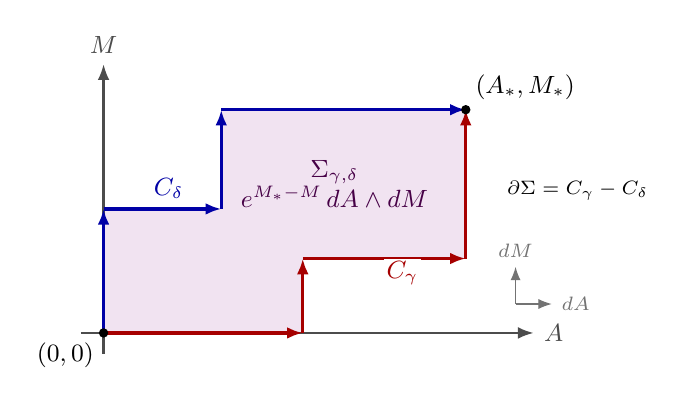
\begin{tikzpicture}[
  x=1.15cm,y=1.05cm,
  axis/.style={-{Latex[length=2mm]},thick,black!70},
  gamma/.style={-{Latex[length=2mm]},very thick,red!65!black},
  delta/.style={-{Latex[length=2mm]},very thick,blue!65!black},
  every node/.style={font=\small}
]
  \coordinate (O) at (0,0);
  \coordinate (g1) at (2.2,0);
  \coordinate (g2) at (2.2,0.9);
  \coordinate (g3) at (4,0.9);
  \coordinate (P) at (4,2.7);
  \coordinate (d1) at (0,1.5);
  \coordinate (d2) at (1.3,1.5);
  \coordinate (d3) at (1.3,2.7);

  \path[fill=violet!11,draw=none]
    (O)--(g1)--(g2)--(g3)--(P)--(d3)--(d2)--(d1)--cycle;
  \draw[axis] (-0.25,0) -- (4.75,0) node[right] {$A$};
  \draw[axis] (0,-0.25) -- (0,3.25) node[above] {$M$};

  \draw[gamma] (O)--(g1);
  \draw[gamma] (g1)--(g2);
  \draw[gamma] (g2)--(g3);
  \draw[gamma] (g3)--(P);
  \draw[delta] (O)--(d1);
  \draw[delta] (d1)--(d2);
  \draw[delta] (d2)--(d3);
  \draw[delta] (d3)--(P);

  \fill (O) circle (1.7pt) node[below left] {$(0,0)$};
  \fill (P) circle (1.7pt) node[above right] {$(A_*,M_*)$};
  \node[red!65!black,fill=white,inner sep=1pt] at (3.3,0.72) {$C_\gamma$};
  \node[blue!65!black,fill=white,inner sep=1pt] at (0.72,1.75) {$C_\delta$};
  \node[align=center,violet!55!black] at (2.55,1.8)
    {$\Sigma_{\gamma,\delta}$\\
     $e^{M_*-M}\,dA\wedge dM$};
  \node[font=\scriptsize,anchor=west] at (4.35,1.72)
    {$\partial\Sigma=C_\gamma-C_\delta$};

  \draw[-{Latex[length=1.7mm]},black!55] (4.55,0.35)--(4.95,0.35)
    node[right,font=\scriptsize] {$dA$};
  \draw[-{Latex[length=1.7mm]},black!55] (4.55,0.35)--(4.55,0.8)
    node[above,font=\scriptsize] {$dM$};
\end{tikzpicture}
\caption{Two charge-compatible ACS histories.  Both paths run from $(0,0)$
to the common charge endpoint $(A_*,M_*)$.  Traversing $C_\gamma$ forward and
$C_\delta$ backward gives the positive boundary of the displayed filling for
the orientation $dA\wedge dM$; the density is weighted by $e^{M_*-M}$.}
\label{fig:acs-compatible-paths-weighted-filling}
\end{figure}

\subsection{Explicit order comparisons}

\paragraph{The elementary rectangle.}
Let
\[
    \gamma=(\mathsf A_p,\mathsf M_q),
    \qquad
    \delta=(\mathsf M_q,\mathsf A_p).
\]
The path \(C_\gamma-C_\delta\) is the positively oriented boundary of the
rectangle \([0,p]\times[0,q]\) when \(p,q>0\).  Direct evaluation and the
weighted-area formula agree:
\begin{align*}
    \tau(\gamma,\delta)
      &=e^q(x+p)-(e^q x+p)\\
      &=p(e^q-1)\\
      &=\int_0^p\int_0^q e^{q-M}\,dM\,dA.
\end{align*}
Thus ``add, then multiply'' minus ``multiply, then add'' is positive under the
orientation fixed in Definition~\ref{def:acs}.  In the flow notation used in
the next chapter, \(p=\mu h\) and \(q=\lambda k\), so the defect is
\[
    \mu h(e^{\lambda k}-1).
\]

\paragraph{A four-step staircase.}
For
\[
    \gamma=(\mathsf A_p,\mathsf M_r,\mathsf A_q,\mathsf M_s),
    \qquad
    \delta=(\mathsf M_r,\mathsf A_p,\mathsf M_s,\mathsf A_q),
\]
the histories have the same total charge \((p+q,r+s)\), but \(\delta\) is not
the temporal reversal of \(\gamma\).  Their evaluations are
\[
    \nu_x(\gamma)=e^{r+s}x+p e^{r+s}+q e^s,
\]
\[
    \nu_x(\delta)=e^{r+s}x+p e^s+q.
\]
Consequently
\begin{equation}
    \tau(\gamma,\delta)
      =p e^s(e^r-1)+q(e^s-1).
    \label{eq:four-step-staircase-torsion}
\end{equation}
For positive \(p,q,r,s\), both terms are positive weighted strips in an ACS
filling.  Formula \eqref{eq:four-step-staircase-torsion} also shows how a later
scale changes the weight of an earlier commutation defect.

\paragraph{Equal charges without reversal.}
The pair
\[
    (\mathsf A_p,\mathsf M_r,\mathsf A_q),
    \qquad
    (\mathsf A_q,\mathsf M_r,\mathsf A_p)
\]
has common charge \((p+q,r)\), and its relative torsion is
\[
    (p-q)(e^r-1).
\]
It may be positive, negative, or zero.  In particular, equal charge does not
determine torsion, while zero torsion does not imply equality of marked
histories.

\subsection{What the ACS forgets}
\label{subsec:p0-acs-forgets}

At the formal level, the map
\[
    \gamma\longmapsto(A_\gamma,M_\gamma)
\]
is an order-forgetting charge homomorphism from concatenated marked histories
to the additive group \(\mathbb R^2\).  It is therefore analogous to an
abelianization map.  This statement concerns the formal charge language only.
It does not identify the symbolic history space with the evaluated affine
group, and it does not assert that either object is a free group without an
additional choice of formal generators and relations.

The content of Theorem~\ref{thm:torsion-stokes} is precisely what survives this
loss of order: the endpoint charges specify a common frame, while the weighted
filling measures the translation defect between two histories.
Section~\ref{sec:p0-contact} retains the current value as a third coordinate and
identifies the infinitesimal form of the same defect with contact curvature.

\subsection{Tearing}
\label{subsec:p0-tearing}

We can now name the phenomenon that the three preceding chapters have been
describing from three sides.  The name is new here, the mathematics is not: it
is the content of Definition~\ref{def:relative-torsion} and
Theorem~\ref{thm:torsion-stokes} read geometrically.

\begin{definition}[Tearing of arithmetic motion]
\label{def:p0-tearing}
Let $\gamma$ and $\delta$ be two add--scale histories of a regular AES that are
scale-compatible in the sense of Section~\ref{sec:p0-acs-tearing}, and let
$\tau(\gamma,\delta)$ be their relative torsion.  The pair is said to \emph{tear}
the AES by $\tau(\gamma,\delta)$: the two histories induce the same linear part,
hence agree on the multiplicative content of the motion, while their additive
content differs by exactly $\tau(\gamma,\delta)$.
\end{definition}

The identification of that scalar defect with an area requires a second
hypothesis, and the two must not be merged.  By
Theorem~\ref{thm:torsion-stokes}, if $\gamma$ and $\delta$ are in addition
*charge-compatible*, then $\tau(\gamma,\delta)$ equals the integral of the
weighted area form over any oriented filling of the closed chain
$C_\gamma-C_\delta$.  For a merely scale-compatible pair the chain
$C_\gamma-C_\delta$ is not closed, because the two paths have different
additive endpoints, so there is no such filling; the scalar defect
\eqref{eq:relative-torsion} remains defined, but it is not yet an area.

Three properties justify treating tearing as a geometric notion rather than a
bookkeeping defect.

\begin{enumerate}
  \item \emph{It exists only relative to the commutativization.}  In the AES
  itself, $\gamma$ and $\delta$ are simply two motions; there is no region
  bounded by them, because the AES is where the two rulers fail to commute.  The
  region appears only after passing to the ACS, and the weight of the filling is
  forced by the evaluation formula \eqref{eq:direct-acs-evaluation}.
  \item \emph{For charge-compatible pairs it is measured, not merely detected.}
  There $\tau(\gamma,\delta)$ is an exact weighted area
  \eqref{eq:torsion-area-integral}; for the elementary rectangle it is
  $\mu h(e^{\lambda k}-1)$, which is the discrete Baumslag--Solitar transport of
  \eqref{eq:p0-bs-relation} read as a defect.
  \item \emph{It is infinitesimally rigid.}  Its density is the constant
  $\mu\lambda$ of \eqref{eq:infinitesimal-order-defect}, which is also the
  bracket coefficient of the arithmetic frame
  \eqref{eq:arithmetic-frame-bracket-on-a}.  Section~\ref{sec:p0-contact}
  shows that this coefficient is the curvature of the specified horizontal
  connection, hence
  that tearing cannot be removed by any local recalibration of the two
  arithmetic directions in which both remain horizontal.
\end{enumerate}

The word \emph{tearing} is chosen because the two-dimensional picture is that of
a surface cut along the two motions: an additive edge and a multiplicative edge
that close up on the level of total charge but not on the level of motion.  The
standard description of a rip in a material is also a pair of paths that agree
far away and separate inside; the arithmetic version of that picture is
Definition~\ref{def:p0-tearing}.  As with ripple geometry, the terminology is
descriptive and asserts nothing beyond the displayed identities; what it adds is
a single name for the phenomenon whose exact measure is the ACS area, whose
infinitesimal density is $\mu\lambda$, and whose carrier in a punctured model is
the subject of Section~\ref{sec:p0-holed}.


\section{The Contact Structure of Tearing}\label{sec:p0-contact}
\input{sections/09-contact-of-tearing.tex}

\section{Beyond Linear Language}\label{sec:p0-beyond-linear}
The picture developed so far is deliberately written in the language of
surfaces, metrics, vector fields, and contact forms.  That language is
convenient, and it is also, in a precise sense, too small.  This section records
two elementary obstructions that explain why we do not take linear language
(manifolds, tangent spaces, Lie groups, and character theory built on modules)
as the foundation of AEG, and it records the alternative that a companion
programme, process geometry, has begun to develop.  The obstructions are
theorems; the alternative is a structural proposal, and the two are kept apart
throughout.

\subsection{Two obstructions to linear language}

The first obstruction concerns the Lie-algebraic reading of the arithmetic
tower.  Addition and multiplication are the first two ranks of that tower: an
additive step moves the assignment by a constant, a multiplicative step scales
it.  On the positive assignment line $a>0$ these two kinds of motion are
generated by
\[
  A=\partial_a,
  \qquad
  M=a\partial_a .
\]
Together with the third rank, multiplication viewed as an endomorphism of
addition, they generate more than a three-dimensional Lie algebra.

\begin{proposition}[The arithmetic generators do not close]
\label{prop:p0-arithmetic-generators}
Let
\[
  A=\partial_a,
  \qquad
  M=a\partial_a,
  \qquad
  P=a\log a\,\partial_a
\]
be defined for $a>0$.  Then
\[
  [A,M]=A,
  \qquad
  [M,P]=M,
  \qquad
  [A,P]=(1+\log a)\partial_a .
\]
The last field does not lie in the real span of $A,M,P$, and the Lie algebra
generated by $A,M,P$ is infinite-dimensional.
\end{proposition}

\begin{proof}
The three brackets are direct: for any smooth $f$,
\[
  [A,M]f=\partial_a\!\left(a f'\right)-a\partial_a f'=f' ,
\]
\[
  [M,P]f=a\partial_a\!\left(a\log a\,f'\right)
        -a\log a\,\partial_a\!\left(a f'\right)
        =a f' ,
\]
\[
  [A,P]f=\partial_a\!\left(a\log a\,f'\right)
        -a\log a\,\partial_a f'
        =\left(1+\log a\right)f' .
\]

For the last claim, suppose first that $(1+\log a)\partial_a=\alpha A+\beta M+\gamma P$
for constants $\alpha,\beta,\gamma$.  Equivalently
$1+\log a=\alpha+\beta a+\gamma a\log a$ for all $a>0$.  Letting
$a\to0^{+}$ makes the left-hand side tend to $-\infty$ while the right-hand
side tends to $\alpha$, a contradiction.  Hence the generated Lie algebra is
strictly larger than $\operatorname{span}\{A,M,P\}$.

More is true.  Since $[A,a^{k}\log a\,\partial_a]
=(k a^{k-1}\log a+a^{k-1})\partial_a$ for every $k\ge1$, the derived algebra
contains $a^{k}\log a\,\partial_a$ for every $k\ge1$.  The coefficient functions
$\{1,a^{k},a^{k}\log a:k\ge1\}$ are linearly independent over $\mathbb R$ on
$a>0$, so these fields span an infinite-dimensional Lie algebra.  A fortiori so
does the algebra generated by $A,M,P$.
\end{proof}

The consequence for the present paper is narrow but decisive.  The two
arithmetic motions of a regular AES are a frame on a surface, and in the basic
hyperbolic model they even exponentiate into the positive affine group.  That is
exactly why $E_0$ is a good first model.  But as soon as the next rank of the
arithmetic tower is admitted, no finite-dimensional Lie group can carry all the
motions: the tower generates an infinite-dimensional algebra, and modelling it
by three coordinates on a finite-dimensional manifold is not an option to be
refused on grounds of taste but a structure that does not exist.  The same
computation, in the calibration of the companion programme, is recorded as the
first strict reason not to model the arithmetic tower as coordinates on an
ordinary finite-dimensional manifold \cite{Yuan2026ProcessGeometry}.

The second obstruction concerns what a *commutative* description can see.  It is
the obstruction that makes the tearing of Section~\ref{sec:p0-acs-tearing}
irreducible rather than an artefact of the presentation.

\begin{proposition}[Commutativization cannot see tearing]
\label{prop:p0-characters-cannot-see-tearing}
Let $\chi$ be any character of the charge group $\mathbb R^2$ of the ACS, and
let $\gamma,\delta$ be charge-compatible add--scale histories with common
charge $(A_*,M_*)$.  Then
\[
  \chi(A_\gamma,M_\gamma)=\chi(A_\delta,M_\delta),
\]
while their evaluation defect is the relative torsion
\[
  \nu_x(\gamma)-\nu_x(\delta)=\tau(\gamma,\delta),
\]
which is independent of $x$ and need not vanish.  Consequently no description
of arithmetic motion by characters of its commutativization can detect tearing.
\end{proposition}

\begin{proof}
The first display is immediate from charge compatibility.  The second is
Proposition~\ref{prop:relative-torsion-independent}.  Nonvanishing is witnessed
by the elementary rectangle: for $\gamma=(\mathsf A_p,\mathsf M_q)$ and
$\delta=(\mathsf M_q,\mathsf A_p)$ one has $\tau(\gamma,\delta)=p(e^{q}-1)$,
which is nonzero whenever $p\ne0$ and $q\ne0$.
\end{proof}

Proposition~\ref{prop:p0-characters-cannot-see-tearing} is the precise sense in
which the linear language fails here, and it is worth stating without
embellishment.  Characters, spectra, and module-theoretic decompositions are
tools for abelian structures; the ACS is the abelian structure naturally
attached to arithmetic motion; and the whole content of the order defect is
*outside* what that abelian structure can resolve.  A description of AEG that
begins from characters therefore begins by discarding the phenomenon the theory
is about.  This is the technical reason for the methodological position taken in
this paper: linear language is used where it is proved to apply
(Sections~\ref{sec:p0-aes}--\ref{sec:p0-contact}), and it is not used as the
ontology of the subject.

\subsection{What process geometry proposes instead}
\label{subsec:p0-beyond-linear-proposals}

The companion programme process geometry develops a vocabulary for exactly this
situation, and the vocabulary is quotable \cite{Yuan2026ProcessGeometry}.  Its
central methodological statement is that geometry is not supplied in advance but
generated by the process and by what its observers can distinguish; and that no
familiar structure may be imported into a *native* description merely because it
is familiar:

\begin{itemize}
  \item geometry enters "because process generation and observer-relative
  distinguishability acquire stable relational, local, and compositional
  structure---not because a manifold, metric, coordinate system, or arithmetic
  model was supplied in advance";
  \item "no level should be imported merely because the next level is
  mathematically familiar";
  \item the public vocabulary deliberately contains *no* group or Lie-group
  hierarchy, *no* general representation hierarchy, and *no* spectrum or
  eigenmode ontology; those "may become justified later, but only after an
  executable vignette requires it";
  \item where a classical mechanism (power series, ordinary polynomial algebra,
  matrix linearization, Fourier or spectral methods, generic computer algebra)
  is used, it must be declared as such and accompanied by a *lowering witness*
  scoped to the exact task and lane, rather than silently acquiring the status
  of native structure.
\end{itemize}

Two features of that programme are relevant to AEG, and only two are claimed
here.

\emph{First, it introduces structure without presupposing a linear carrier.}  A
process is a generation rule; a history is what that rule produces; a task
selects which distinctions matter; and the resulting quotient, when it is
stable, may be *objectified* into a new primitive of the next rank.  The
vocabulary is deliberately non-linear: it speaks of presentations, semantic
compression, rank raising, and rank lowering, and its stated obligations are
compositional (a higher-rank composition must remain interpretable at the lower
rank) rather than algebraic in the module-theoretic sense.

\emph{Second, it records an obstruction of the same kind as
Proposition~\ref{prop:p0-characters-cannot-see-tearing}.}  Its finite-family
layer introduces families with a parameter composition law, together with
one-dimensional response objects, and then states plainly that such
one-dimensional scalar response is *not* sufficient to encode the additive
--multiplicative interaction while retaining a nontrivial translation response.
The layer stops at that obstruction instead of enlarging the ambient linear
structure; the accompanying declaration says that the object "does not require
inverses, topology, Haar measure, Lie algebra, commutativity, or even a group
structure".  This is the same lesson as
Proposition~\ref{prop:p0-characters-cannot-see-tearing}, arrived at from the
side of computation.

\subsection{Exact calibrations that meet this paper's laws}

The proposals above would be of little use if they did not meet the identities
proved here.  They do, and in one case the match is literal.

\begin{enumerate}
  \item \emph{The discrete transport law.}  In the calibration of the companion
  programme, the objectified multiplication acts on translation by
  \[
    D_kT_a=T_{ka}D_k ,
  \]
  and the mixed language generated by both is the positive affine monoid
  $\mathbb Z\rtimes\mathbb N_{>0}$.  This is exactly the relation
  \eqref{eq:p0-bs-relation} of Section~\ref{sec:p0-aes}, read in the equivalent
  direction convention:
  \[
    \mathsf Y_k\,\mathsf X_s\,\mathsf Y_k^{-1}=\mathsf X_{ks},
  \]
  with $D_k=\mathsf Y_k$ and $T_a=\mathsf X_a$.  The two programmes therefore
  meet at the same discrete law, one derived from the arithmetic grid and the
  other from a rank-lowering obligation.
  \item \emph{The infinitesimal transport law.}  In the continuous form the same
  structure appears as $S_sT_t=T_{e^st}S_s$ together with the algebra relation
  $[A,M]=A$ for $A=\partial_a$ and $M=\partial_v+a\partial_a$.  This is the
  affine structure equation already used in Section~\ref{sec:p0-aes}.  It must
  not be confused with the horizontal bracket
  \eqref{eq:horizontal-noncommutation}: the latter is the curvature of the
  horizontal distribution in the three-dimensional contact model of
  Section~\ref{sec:p0-contact}, whereas $[A,M]=A$ is a bracket on the base
  algebra of the two arithmetic motions.  The two are related --- both have the
  same coefficient $\mu\lambda$ in the arithmetic frame --- but they are
  different objects, and the identification is not made here.
  \item \emph{Non-integrability in a second calibration.}  The companion
  programme also records the exact local obstruction
  \[
    \vartheta=dz-x\,dy,
    \qquad
    X=\partial_x,
    \qquad
    Y=\partial_y+x\partial_z,
    \qquad
    [X,Y]=\partial_z,
    \qquad
    \vartheta([X,Y])=1 .
  \]
  Since $d\vartheta=-dx\wedge dy$, one has
  $\vartheta\wedge d\vartheta=dx\wedge dy\wedge dz\ne0$: $\vartheta$ is a
  contact form whose kernel does not close, exactly as for the arithmetic
  contact form \eqref{eq:arithmetic-contact-form}, of which $\vartheta$ is the
  normalization obtained by setting $\lambda=1$, $\mu=1$ and integrating the
  additive direction.  The same non-integrability pattern therefore appears in
  a calibration where no arithmetic assignment is present at all.
\end{enumerate}

These three items are exact computations, not proposals.  Their status is
nevertheless local to their own calibration: they are recorded in a research
repository whose own maturity labels are, for the items cited, of the kind
"precise conjecture" and "research calibration", and this paper does not promote
them.

\subsection{Status and non-claims}

For the avoidance of doubt, this section claims the following and nothing more.

\begin{itemize}
  \item Proposition~\ref{prop:p0-arithmetic-generators} and
  Proposition~\ref{prop:p0-characters-cannot-see-tearing} are proved above, by
  elementary computation, in this paper.
  \item The vocabulary of Subsection~\ref{subsec:p0-beyond-linear-proposals} is a
  \emph{structural proposal}: it is a way of organizing the construction of
  non-linear descriptions, imported from a companion programme and used here as
  a language, not as a theorem about AEG.
  \item This section does not claim that manifolds, metrics, Lie groups,
  modules, or characters are illegitimate in AEG.  Sections~\ref{sec:p0-aes},
  \ref{sec:p0-acs-tearing}, and~\ref{sec:p0-contact} use all of them, and use
  them with proofs.  What is refused is their status as ontology: no linear
  structure is imported into a foundational claim without a derivation of its
  transport at the arithmetic rank in question.
  \item This section does not claim any universality of arithmetic-generated
  geometry, and it does not import the companion programme's own open
  conjectures.  Where that programme states that a claim is not established, the
  same claim is not established here.
  \item No efficiency, complexity, or approximation statement is made.  The two
  propositions above are structural obstructions, and an obstruction is not a
  lower bound: no conclusion about computational cost follows from them, in
  either direction.
\end{itemize}


\section{Holed Arithmetic Expression Spaces and the Language of Tearing}\label{sec:p0-holed}
The geometry of Section~\ref{sec:p0-aes} is developed on the basic model, which
is complete and unpunctured: $\mathfrak E_0$ has no point at which the
arithmetic structure fails.  (The one-puncture model $\mathfrak E_1$ of
Example~\ref{ex:p0-e1-model} already leaves the regular category, and is the
case this chapter generalizes.)  This final chapter records the opposite
situation, which arose in the most recent
exploratory work of the programme, and the vocabulary that has been proposed for
it.  The mathematical content of the chapter is deliberately modest: one
definition, one exact local computation, and a register of six computed
witnesses, each with its own status.  The interpretive reading of those
witnesses --- the language of tearing --- is presented as a structural proposal,
and Subsection~\ref{subsec:p0-holed-nonclaims} lists what is not established.

\subsection{Punctured arithmetic expression spaces}
\label{subsec:p0-holed-definition}

\begin{definition}[Punctured arithmetic expression space]
\label{def:p0-punctured-aes}
Let $\overline M$ be an oriented smooth surface, let $S\subset\overline M$ be a
finite set of points, and put $M=\overline M\setminus S$.  Suppose given a
smooth Riemannian metric $g$ on $M$, a function $a:M\to\mathbb R$ that is smooth
on $M$, and constants $\mu\ne0$, $\lambda$, such that
\begin{enumerate}
  \item $(M,g,a;\mu,\lambda)$ is a regular AES in the sense of
  Definition~\ref{def:regular-aes}, and
  \item for every $p\in S$, no neighbourhood $U$ of $p$ in $\overline M$ admits
  extensions of $g|_{U\cap M}$ and $a|_{U\cap M}$ to smooth data
  $\widetilde g,\widetilde a$ on $U$ for which
  $(U,\widetilde g,\widetilde a;\mu,\lambda)$ is a regular AES.
\end{enumerate}
Then $(\overline M,S,g,a;\mu,\lambda)$ is called a \emph{punctured arithmetic
expression space}, and the points of $S$ are its \emph{punctures}.  When
$|S|=k$ we write $\mathfrak E_k$ for it, in the descriptive sense of
Convention~\ref{conv:p0-model-labels}.
\end{definition}

The ambient surface and the data are deliberately separated: the regular AES is
given only on the punctured surface $M$, so that condition (ii) is a genuine
requirement rather than a contradiction.  A puncture is not any point that has
been deleted, but a point at which the regular structure genuinely cannot be
continued.  This is the finite-point case of the singular arithmetic expression
space of Paper~I; the general singular theory, the classification of singular
germs, and everything concerning tubes, braids, and knot invariants belong to
Paper~I and Paper~III.  The notion is specialized here for one reason only: the
arithmetic motions of Subsection~\ref{subsec:p0-point-paths} are defined on the
punctured surface, and the question of what happens to them at a puncture is a
question about AES.

The first example is the one-puncture model of Example~\ref{ex:p0-e1-model}: the
unit disc with the complete Poincar\'e metric and the radial assignment
$a_{\mathbb D}=\frac{2\mu}{\lambda}\rho/(1-\rho^2)$, whose metric extends
smoothly across the centre while the assignment does not.  There $S=\{0\}$ and
the regular locus is $\mathbb D\setminus\{0\}$.  Two features of that example
are worth recording here, because they are typical of punctured models.  First,
the extended metric is complete on $\mathbb D$ while its restriction to
$\mathbb D\setminus\{0\}$ is \emph{not} complete: the puncture is at finite
distance from every interior point, so the incompleteness is caused by the
deletion and not by the geometry.  Second, the assignment has a finite limit at
the puncture (here $0$) but no $C^1$ extension, so the failure is a failure of
differentiability rather than of continuity.  Both statements are verified in
Paper~I together with the model.

\subsection{The local shape of a puncture}
\label{subsec:p0-holed-tangent-cone}

A puncture is not merely a missing point; at least in the example that has been
computed in detail, it carries a definite local shape.  The following statement
is exact.

\begin{proposition}[Tangent cone of the four limiting circles]
\label{prop:p0-puncture-tangent-cone}
Fix $\rho>0$ and consider the four circles through the origin
\[
  C_\pm:\ x^2+y^2\mp2\rho y=0,
  \qquad
  D_\pm:\ x^2+y^2\mp2\rho x=0 .
\]
Write $S_2=x^2+y^2$ and let
\[
  P=\bigl(S_2^2-4\rho^2y^2\bigr)\bigl(S_2^2-4\rho^2x^2\bigr)
\]
be the defining polynomial of their union.  Then
\[
  P=S_2^4-4\rho^2S_2^3+16\rho^4x^2y^2 ,
\]
so the lowest-degree homogeneous part of $P$ is $16\rho^4x^2y^2$.  Consequently
the tangent cone of the union at the origin is
\[
  (xy)^2=0 ,
\]
that is, the two coordinate axes, each with multiplicity two.
\end{proposition}

\begin{proof}
The four circles are $S_2=\pm2\rho y$ and $S_2=\pm2\rho x$, whose defining
polynomials are $S_2^2-4\rho^2y^2$ and $S_2^2-4\rho^2x^2$ respectively; the
product is $P$.  Expanding,
\[
  \bigl(S_2^2-4\rho^2y^2\bigr)\bigl(S_2^2-4\rho^2x^2\bigr)
  =S_2^4-4\rho^2S_2^2(x^2+y^2)+16\rho^4x^2y^2
  =S_2^4-4\rho^2S_2^3+16\rho^4x^2y^2 ,
\]
since $S_2^2(x^2+y^2)=S_2^3$.  The terms have degrees eight, six, and four, so
the lowest-degree part is $16\rho^4x^2y^2$, whose zero set is $xy=0$ counted
twice.
\end{proof}

Two remarks, both used below.  First, the two circles of the same family are
tangent at the origin, so the origin is a degenerate point of each family, while
circles of different families cross there with tangent lines $x=0$ and $y=0$;
the tangent cone is the union of those two lines.  Second, the tangent cone is
*reducible with multiplicity*: it is the square of a product of two distinct
linear forms.

No arithmetic expression space is attached to this configuration in this paper.
The four circles are an explicit curve configuration whose tangent cone can be
computed exactly, and nothing more is claimed: in particular they are not
asserted to be the limiting circles of any AES metric or assignment, and the
origin is not asserted to be a puncture in the sense of
Definition~\ref{def:p0-punctured-aes}.  Constructing data $(g,a)$ on a
neighbourhood of the origin for which this configuration is natural, and for
which the origin is non-extendable, is recorded as the first problem of
Subsection~\ref{subsec:p0-holed-open}.
The computation is recorded in the exploration register of the
programme \cite{Yuan2026AEGHoleRegister}; the identity above is verified here
directly.

\subsection{Tearing at a puncture}
\label{subsec:p0-tearing-at-puncture}

The tearing of Definition~\ref{def:p0-tearing} is a defect between two motions
of a space.  On a punctured space a further question arises: the motions
themselves need not be extendable across the puncture, so a comparison of two
motions may have to be performed around it rather than through it.  This
subsection records that question and what is known about it; it proves nothing
beyond the definitions.

Let $(\overline M,S,g,a;\mu,\lambda)$ be a punctured AES and let $p\in S$.  A
motion of the punctured surface is a path in $M=\overline M\setminus S$, and two
motions that approach $p$ from different directions need not have limits related
by any regular motion of the punctured part: the assignment and the metric are
defined only on $M$.  The following two questions are therefore well posed.

\begin{enumerate}
  \item \emph{Does comparison require a detour?}  Two bounded motions with the
  same charge whose paths cannot be deformed into one another in $M$ while
  keeping their charges: is their relative torsion still given by an ACS area,
  and if so in which filling class?  The frame witness of
  Subsection~\ref{subsec:p0-holed-witnesses} is the computed instance that makes
  the question concrete, because there a closed loop in one coordinate is open
  in another.
  \item \emph{Does comparison require a cut?}  If the punctures are stipulated
  rather than derived, then the family of comparisons depends on that
  stipulation.  The gluing witness of the same subsection exhibits a whole
  family of cuts whose invariants are exhausted by a permutation, so the cut
  carries more information than the topology it produces.
\end{enumerate}

Neither question is answered here.  What can be said now is only where the
measurement must be performed: the measured value of tearing is the ACS area of
Theorem~\ref{thm:torsion-stokes}, which is a statement about add--scale
histories and therefore does not itself refer to the puncture; a comparison
across a puncture has to leave the punctured surface, either by passing to the
charge plane or by going around the puncture, and deciding which of the two is
canonical is recorded as the second problem of
Subsection~\ref{subsec:p0-holed-open}.

\subsection{Six computed witnesses}
\label{subsec:p0-holed-witnesses}

The exploratory work recorded in \cite{Yuan2026AEGHoleRegister} produced six
separately computed statements about punctured configurations.  They are
reproduced here in the register's own order, each with its exact content and its
status.  None of them is promoted by appearing in this paper: the register
carries no authoritative status, and the items below are classified according to
the labels of this repository.

\begin{enumerate}
  \item \emph{A topological witness.}  Cut a disc carrying four right-angle
  sectors along the two diagonal seams and the four coordinate rays; eight
  triangular pieces result, each with a left radial edge, an outer arc, and a
  right radial edge.  Regluing is a permutation $\sigma$ of the eight left edges
  onto the eight right edges.  If $C$ is the number of cycles of $\sigma$, then
  the centre vertex has $C$ orbits, the outer vertices form eight orbits, and
  $V=C+8$, $E=16$, $F=8$, whence
  \[
    \chi=V-E+F=C=b ,
  \]
  the number of boundary components.  Consequently every gluing of this family
  produces either one disc or a disjoint union of $C$ discs, and the compact
  three-holed sphere ($\chi=-1$ with three boundary components) is unreachable
  in this family.  A surface of Euler characteristic $-1$ is obtained instead by
  removing two points from the disc: it has one boundary component, two
  punctures, and hence three ends, so its Euler characteristic agrees with that
  of the compact pair of pants while its boundary structure does not.  An
  exhaustive check of all $40320$ permutations confirms the
  distribution $5040,13068,13132,6769,1960,322,28,1$ for $C=1,\ldots,8$.
  \emph{Status:} the identity $\chi=C$ is elementary and provable as above; the
  enumeration is a computationally verified example.  The topological
  conclusion holds for the stated gluing rule, not for arbitrary gluings of the
  eight pieces.

  \item \emph{A combinatorial witness.}  If three components interact pairwise,
  the interaction sites are the three unordered pairs, and each site carries two
  directions of exchange, giving six directed transitions in total.
  \emph{Status:} counting, given the definition of a hole as an interaction
  site.  The definition is a choice, not a theorem.

  \item \emph{A frame witness.}  Let the state of a three-component frame be
  $(c,\sigma,\varphi)$ with component label $c\in\mathbb Z_3$, direction
  $\sigma\in\{\pm1\}$, and phase $\varphi\in\mathbb Z_4$, and let one step act by
  \[
    (c,\sigma,\varphi)\longmapsto(c+\sigma,\sigma,\varphi+\sigma).
  \]
  Since $\gcd(3,4)=1$, the Chinese remainder theorem identifies
  $(c,\varphi)$ with a single counter $k$ modulo $12$, and the orbit of each
  direction has length $12$.  Within one such orbit the component label
  advances in the direction $\sigma$, so the transitions realized are the three
  pairs of that direction, each occurring four times --- once per phase class.
  The six directed transitions of the combinatorial witness therefore appear
  four times each only over the two orbits together, that is, over $24$ steps;
  a single $12$-step orbit cannot contain $24$ transitions.  Since one full
  phase period is four steps and $4\equiv1\pmod3$, one period of the phase
  returns the phase to its initial value while advancing the component label by
  \[
    c\longmapsto c+\sigma \pmod 3 ;
  \]
  for the fixed direction $\sigma=+1$ this is the advance by one used in the
  register, and for $\sigma=-1$ it is the advance by two.  In either case the
  phase loop is not closed in the total state: its monodromy is the generator
  $-\sigma$ of $\mathbb Z_3$.  \emph{Status:} exact arithmetic (Chinese
  remainder theorem), verified exhaustively on the two $12$-state orbits and by
  replay.

  \item \emph{An observer witness.}  Let a frame be described by an angle
  $\theta$ and three joint offsets $\delta_1,\delta_2,\delta_3$, and let the
  residuals available to an observer be
  \[
    r_i=\bigl|2\sin\delta_i\bigr| \quad (i=1,2,3),
    \qquad
    r_4=\bigl|2\sin\bigl(2\theta+\tfrac12(\delta_1+\delta_2+\delta_3)\bigr)\bigr| .
  \]
  All four residuals vanish exactly at the ideal frame
  $(\theta,\delta)=(\pi/2,0,0,0)$.  Suppose an observer sees only residuals of
  magnitude at least $\varepsilon$, and that an iterative procedure stops as
  soon as every visible residual is below that threshold.  At the halt one then
  has the following bound.  From $r_i<\varepsilon$ we get
  $|\delta_i|<\arcsin(\varepsilon/2)=\varepsilon/2+O(\varepsilon^3)$, and from
  $r_4<\varepsilon$ together with
  $r_4=\bigl|4(\theta-\pi/2)+(\delta_1+\delta_2+\delta_3)\bigr|+O(\lVert(\theta-\pi/2,\delta)\rVert^2)$
  we get
  \[
    \bigl|\theta-\pi/2\bigr|
    <\frac58\,\varepsilon+O(\varepsilon^2).
  \]
  The halting offset is therefore of order $\varepsilon$ and decreases linearly
  in $\varepsilon$; it is not zero, and it is the best that a procedure obeying
  this stopping rule can report.  \emph{Status:} the residual functions, their
  exact common zero at the ideal frame, and the bound are proved above.  The
  particular iteration counts and offsets recorded in the register depend on the
  implementation of the update step, which the register does not fix, and they
  are accordingly \emph{not} reproduced here.  The witness is \emph{not} an
  obstruction: nothing in the computation shows that no procedure can do better,
  and the exact zero of the residuals at the ideal frame shows the opposite.

  \item \emph{A semantic witness.}  Model the three interaction sites by
  vocabularies built from four terms common to all three components, four
  further control terms distributed over the pairs as two, one, and one, and
  three terms private to the individual components (which therefore enter no
  site vocabulary).  The three site vocabularies then have sizes
  \[
    6=4+2,\qquad 5=4+1,\qquad 5=4+1 .
  \]
  Filling the three sites independently --- one word chosen from
  each site's own vocabulary --- gives $6\cdot5\cdot5=150$ possibilities;
  filling them so that the same core word is used at all three sites gives
  $4^3=64$.  The difference $86$ is carried by the adapters at the sites.  On
  the control layer the pairwise intersections are non-empty while the common
  intersection is empty; on the full vocabularies the common intersection is the
  four-term core, so the emptiness statement is layer-dependent.
  \emph{Status:} the arithmetic is verified given the model; the model is a
  modelling choice, and the "Borromean" description is an analogy with no
  link-theoretic content.

  \item \emph{A phase-geometry witness.}  With components at phases
  $\{0,+1,-1\}$ modulo $n$, a forward motion of $k$ steps and a reverse motion of
  $m$ steps meet exactly when $k+m\equiv0\pmod n$.  A meeting phase different
  from the three component phases exists precisely for $n\ge4$; at $n=4$ it is
  the first case in which the meeting is simultaneously balanced ($k=m$) and
  antipodal ($\varphi=n/2$), namely $k=m=2$, $\varphi=2$.  \emph{Status:}
  computationally verified example over the stated finite model, exhaustive for
  $n=3,\ldots,8$.  The value $n=4$ is minimal, not unique: $n=6$ and $n=8$ also
  admit balanced antipodal meetings.
\end{enumerate}

\begin{remark}[Register bookkeeping]
\label{rem:p0-holed-register-bookkeeping}
The exploration register introduces these items as five classes while tabulating
six rows; the sixth row is the phase-geometry witness listed last above.  This
paper follows the table and counts six, recording the discrepancy rather than
resolving it silently \cite{Yuan2026AEGHoleRegister}.
\end{remark}

\subsection{What the witnesses do not establish}
\label{subsec:p0-holed-nonclaims}

The register's own summary sentence is that a hole "is not a defect to be
removed but the position that carries exchange".  That sentence is the
motivation for this chapter, and it is not proved by any of the six witnesses.
The following list of non-claims is part of the content of this section.

\begin{itemize}
  \item No witness shows that punctures are unavoidable in AES.  The witnesses
  are about chosen finite models: a chosen gluing family, a chosen frame, a
  chosen vocabulary, a chosen stopping rule.  Changing the model changes the
  count, and the register says so for its own semantic witness.
  \item No witness establishes an obstruction of AEG.  The monodromy of the
  frame witness is a monodromy of a stipulated finite flow; the calibration
  witness is a property of a stipulated halting rule; the gluing witness is a
  statement about one gluing family.
  \item The $\mathbb Z_3$ monodromy of the frame witness is not identified with
  any $\mathbb Z_4$ twist of sheet labels appearing elsewhere in the register.
  Those are different groups, and no computation in the register relates them;
  the identification asserted there is recorded as unproved.
  \item The word "hole" in this chapter means a puncture in the sense of
  Definition~\ref{def:p0-punctured-aes}, or an interaction site in the sense of
  the combinatorial witness.  It is not the "one-hole context" of
  Section~\ref{sec:p0-expansion}, which is a placeholder in an expression, and
  the two must not be conflated.
  \item The engineering study that accompanies the register is explicitly
  recorded by its author as an analogy and not as a mathematical assertion; one
  of its three language prototypes was never compiled.  It contributes
  motivation only.
  \item Nothing here changes the status of Paper~I's regular-zero theorems or of
  Paper~III's singular theory.  A punctured AES is a specialization of the
  singular notion, and its classification is not attempted.
\end{itemize}

\subsection{Open problems}
\label{subsec:p0-holed-open}

The register closes with the author's own verdict that this route is not yet
free, for three reviewable reasons: the family of cuts depends on a chosen
permutation, the covering sheets are defined by the cut, and the graded
description depends on an externally supplied frame.  It registers three
directions that have not been attempted, and they are the natural open problems
of this chapter.

\begin{enumerate}
  \item Replace the tangent cone of Proposition~\ref{prop:p0-puncture-tangent-cone}
  by the formal neighbourhood of the puncture: compute the successive jets at
  $p$ and test whether the description ceases to depend on the choice of tangent
  directions.
  \item Blow up the puncture and rewrite the cut-and-glue construction as a
  canonical construction on the exceptional divisor, so that the seam is
  replaced by a construction the data itself determines.
  \item Replace the cut-and-glue calculus by an operadic composition, in which
  the gluing of punctured surfaces is intrinsic and contains no chosen seam.
\end{enumerate}

Each of these is a programme, not a result.  Three further problems arise
directly from the discussion above, and are recorded with their own labels.

\begin{enumerate}
  \item \label{op:p0-four-circle}\emph{Attach AES data to the four-circle
  configuration.}  Construct a surface $\overline M$, a finite set $S$ containing
  the origin, and data $(g,a)$ on $\overline M\setminus S$ such that
  $(\overline M,S,g,a;\mu,\lambda)$ is a punctured AES in the sense of
  Definition~\ref{def:p0-punctured-aes}, such that the four circles (or their
  limiting arcs under $g$) arise naturally from $a$ or from the arithmetic
  motions, and such that the origin is non-extendable.  Until such a
  construction exists, Proposition~\ref{prop:p0-puncture-tangent-cone} is a
  statement about a curve configuration and not about any AES.
  \item \label{op:p0-canonical-punctures}\emph{Make the comparison across a
  puncture canonical.}  Decide whether a relative torsion across a puncture is
  measured by an ACS area, by a holonomy around the puncture, or by neither, and
  in the first case determine the admissible filling classes.
  \item \emph{Make the puncture set canonical.}  Decide whether the set $S$ of
  Definition~\ref{def:p0-punctured-aes} can be determined by the arithmetic data
  rather than stipulated, and whether it is unique when it can.  This is the
  first unfinished item of the exploration register's own programme.
\end{enumerate}

A solution of any of them would turn the language of this chapter from a
description into a theory; the earlier prelude's question, whether a punctured
model carries a ripple structure that survives at the puncture, is a fourth and
independent problem of the same kind.


\section{Interfaces to Papers I--IV}\label{sec:p0-interface}
This paper was enlarged to become the geometric foundation of the series.  The
division of labour between Paper~0 and Paper~I is fixed by the authoritative
amendment `governance/00b-paper-0-geometric-foundation-amendment.md`, and this
section records the resulting interface without restating either paper's
theorems.

\subsection{What Paper 0 establishes}

The proved spine of this paper is
\[
\begin{gathered}
  \text{left and right comb grammars}
  \longrightarrow
  \text{slot-$(1)$/slot-$(2)$ one-hole maps},\\
  \text{distributive expansion}
  \longrightarrow
  \text{same operator, different charges},\\
  \text{arithmetic motions on an AES}
  \longrightarrow
  \text{point path in } \mathfrak E_0,\\
  \text{projective operator}
  \longrightarrow
  \text{pole, fixed points, ripple pencil},\\
  \text{affine cocycles}
  \longrightarrow
  \text{relative defect}
  \longrightarrow
  \text{ACS weighted area},\\
  \text{contact form}
  \longrightarrow
  \text{non-integrable horizontal distribution}
  \longrightarrow
  \text{curvature } \mu\lambda,\\
  \Aff(1,K)=\Stab(\infty)
  \subset
  \PGL_2(K).
\end{gathered}
\]
The paper also supplies four laboratories: the basic hyperbolic model
$\mathfrak E_0$, the one-puncture model $\mathfrak E_1$, the pulled-back
horocycle pencil, and the three-dimensional contact model.  The finite
geometric-series and continued-fraction examples are exact at every truncation;
their infinite values are asserted only under the stated formal or analytic
convergence hypotheses.

Two statements in the paper are not theorems about AES and are labelled as
proposals where they occur: the descriptive name *ripple geometry* for the dual
reading of Section~\ref{sec:p0-ripples}, and the language of *tearing* of
Section~\ref{sec:p0-acs-tearing} together with the punctured reading of
Section~\ref{sec:p0-holed}.  Both rest on proved computations --- the
line-to-circle theorem, the weighted torsion--Stokes theorem, and the contact
curvature --- and neither claims a new isomorphism class of geometry.

\subsection{What remains in Paper I}

Paper~I begins one level earlier and keeps the history layer.  It retains
responsibility for:

\begin{enumerate}
  \item the intrinsic dependency-poset classification of all sequential binary
  trees, including mixed slot words;

  \item marked planar sequential trees and bounded/free marked spinal
  histories, with operand-slot chirality, mirror, temporal reversal, and path
  inverse kept distinct;

  \item projective evaluation of chronological marked histories, including
  ordinary-domain data and the affine sector;
  
  \item the $q=4$ Hecke sublanguage and its history-level relations;

  \item the regular-zero theorems, the complete splitting theorem, the
  foundational definition of a singular arithmetic expression space, the
  verified isolated-zero model, and the smooth parameter-family zero-set lemma;

  \item the interfaces to Papers~II, III, and~IV.
\end{enumerate}

Paper~I states the definition of a regular AES and its canonical frame as a
concise imported interface, because its zero theorems are stated in those terms;
everything else that moved here is referenced rather than repeated.  The earlier
version of that interface, which ran in the opposite direction, is superseded.

\subsection{The dependency architecture}

The series dependency is
\[
  \boxed{
  \text{Paper 0}
  \longrightarrow
  \text{Paper I}
  \longrightarrow
  \{\text{Papers II, III, IV}\}.
  }
\]
The first arrow exports the following interfaces:

\begin{center}
\renewcommand{\arraystretch}{1.3}
\begin{tabular}{ll}
\toprule
Paper 0 object & use in later papers \\
\midrule
comb and slot conventions & operand-slot chirality on sequential spines \\
distributive expansion & comparison of expansions with equal operator \\
regular AES and canonical frame & imported definition for zero theory \\
arithmetic motions and $\mathfrak E_0$ & model for analysis and for the flow \\
one-puncture model $\mathfrak E_1$ & first punctured instance \\
point path & bounded marked-history evaluation in the affine sector \\
ripple pencil and pole & motivation for bilateral projective continuation \\
affine cocycles & discrete order defect \\
ACS and relative torsion & global torsion and its measures \\
contact form and horizontal curvature & horizontal calculus and function theory \\
tearing and punctured spaces & vocabulary for singular and resource questions \\
\bottomrule
\end{tabular}
\end{center}

Papers~II and~III import the regular-AES definition, the canonical frame, the
basic hyperbolic model, the contact model, and the elementary bilateral
operators from this paper; they do not redefine them.  Paper~IV imports the
history layer from Paper~I and the affine torsion from this paper.

\subsection{Open extensions}

Several genuine problems remain, and they are recorded here rather than
advertised as results.

\begin{enumerate}
  \item Construct a projective analogue of the affine arithmetic expression
  space in which the pole and the ripple pencil are intrinsic rather than chosen
  through one upper-half-plane chart, and decide which path or ripple data
  descend through relations among history words.

  \item Decide whether the contact structure of Section~\ref{sec:p0-contact}
  admits a canonical compatible structure beyond the horizontal distribution,
  and if so which.  Neither a complex structure nor a horizontal metric is
  determined by the contact form alone.

  \item Determine whether the choice of punctures in Section~\ref{sec:p0-holed}
  can be made canonical, and whether a punctured model carries a ripple
  structure that survives at the puncture; the three registered programmes of
  Subsection~\ref{subsec:p0-holed-open} are the concrete routes.

  \item Extend the one-hole analysis to multi-wire expression networks while
  retaining ordinary-domain, pole, and fixed-point information, and develop a
  controlled theory of infinite arithmetic expressions that separates formal,
  analytic, projective, and computational convergence.

  \item Determine whether the non-linear algebraic structures proposed in
  Section~\ref{sec:p0-beyond-linear} can be defined intrinsically for AES, so
  that the two proved obstructions of that section are replaced by a positive
  description rather than a refusal.
\end{enumerate}

None of these problems is solved merely by the matrix representation or by the
existence of the contact form.  The stable conclusion of the present paper is
more elementary: the four arithmetic operations act as motions of one space,
their order defect is measured in the commutativization of that space, and the
contact structure of the same defect is what prevents the two motions from being
calibrated independently.


\appendix
\section{Elementary Calculations}\label{app:p0-calculations}
This appendix records calculations used in the main text.  They are included
to keep the elementary claims reproducible and to fix chronology and sign
conventions.

\subsection{Chronological products and one-hole recursion}

Let
\[
  F_k(z)=\frac{A^{(k)}z+B^{(k)}}{C^{(k)}z+D^{(k)}}
\]
have matrix representative
\[
  M_k=
  \begin{pmatrix}
    A^{(k)}&B^{(k)}\\
    C^{(k)}&D^{(k)}
  \end{pmatrix}.
\]
If $F_1$ acts first, the two-step action is
\[
  F_2(F_1(z)),
\]
and direct substitution gives the matrix $M_2M_1$.  Induction therefore gives
\[
  F_k\circ\cdots\circ F_1
  \longleftrightarrow
  M_k\cdots M_1.
\]
This is the convention used in \eqref{eq:p0-prefix-matrices}.

For affine matrices
\[
  M_k=\begin{pmatrix}\alpha_k&\beta_k\\0&1\end{pmatrix},
  \qquad
  P_{k-1}=\begin{pmatrix}A_{k-1}&B_{k-1}\\0&1\end{pmatrix},
\]
one has
\[
  M_kP_{k-1}
  =\begin{pmatrix}
     \alpha_kA_{k-1}&\alpha_kB_{k-1}+\beta_k\\
     0&1
   \end{pmatrix},
\]
which is the recursion \eqref{eq:p0-affine-prefix-recursion}.

\subsection{The ripple circle calculation}

For
\[
  F(z)=\frac{Az+B}{Cz+D},
  \qquad
  \Delta=AD-BC>0,
\]
one computes
\begin{align*}
  F(z)-\overline{F(z)}
  &=\frac{(Az+B)(C\bar z+D)-(A\bar z+B)(Cz+D)}{|Cz+D|^2}\\
  &=\frac{(AD-BC)(z-\bar z)}{|Cz+D|^2}.
\end{align*}
Dividing by $2i$ gives
\[
  \im F(z)=\frac{\Delta\,\im z}{|Cz+D|^2}.
\]
Writing $z=x+iy$ and imposing $\im F(z)=t$ gives
\[
  \Delta y=t\bigl((Cx+D)^2+C^2y^2\bigr).
\]
When $C\ne0$, division by $tC^2$ yields
\[
  \left(x+\frac DC\right)^2+y^2
  -\frac{\Delta}{tC^2}y=0,
\]
and completing the square yields \eqref{eq:p0-ripple-circle}.

For $J(z)=-1/z$, one has $A=D=0$, $B=-1$, $C=1$, and
$\Delta=1$.  Hence
\[
  x^2+\left(y-\frac1{2t}\right)^2=\left(\frac1{2t}\right)^2.
\]

\subsection{Powers of an affine map}

Let $T(z)=az+b$ with $a\ne0$.  Matrix multiplication gives
\[
  \begin{pmatrix}a&b\\0&1\end{pmatrix}^n
  =\begin{pmatrix}
     a^n&b(1+a+\cdots+a^{n-1})\\
     0&1
   \end{pmatrix}.
\]
If $a\ne1$, this is
\[
  \begin{pmatrix}
     a^n&b(1-a^n)/(1-a)\\
     0&1
   \end{pmatrix}.
\]
Writing $q=b/(1-a)$, the induced map becomes
\[
  T^n(z)=a^nz+q(1-a^n)=q+a^n(z-q).
\]
If $a=1$, the matrix power is
\[
  \begin{pmatrix}1&nb\\0&1\end{pmatrix},
\]
so $T^n(z)=z+nb$.

For the geometric-series update $T_r(s)=rs+1$, apply the same formula with
$a=r$, $b=1$, and $s=0$:
\[
  T_r^n(0)=\frac{1-r^n}{1-r}
\]
when $r\ne1$.

\subsection{Continued-fraction matrices}

Let
\[
  F_k(z)=a_k+\frac{b_k}{z},
  \qquad
  M_k=\begin{pmatrix}a_k&b_k\\1&0\end{pmatrix},
  \qquad b_k\ne0.
\]
Write
\[
  P_k=M_k\cdots M_1
     =\begin{pmatrix}p_k&r_k\\q_k&s_k\end{pmatrix}.
\]
Then
\[
  P_k
  =\begin{pmatrix}a_k&b_k\\1&0\end{pmatrix}
   \begin{pmatrix}p_{k-1}&r_{k-1}\\q_{k-1}&s_{k-1}\end{pmatrix}
  =\begin{pmatrix}
      a_kp_{k-1}+b_kq_{k-1}&a_kr_{k-1}+b_ks_{k-1}\\
      p_{k-1}&r_{k-1}
    \end{pmatrix}.
\]
Thus
\[
  q_k=p_{k-1},
  \qquad
  p_k=a_kp_{k-1}+b_kp_{k-2},
\]
with the analogous recurrence for the second column.  The $k$th truncation at
an initial value $z_0$ is
\[
  F_k\circ\cdots\circ F_1(z_0)
  =\frac{p_kz_0+r_k}{q_kz_0+s_k}.
\]
An ordinary truncation is admissible precisely when each intermediate
denominator is nonzero; the projective formula also records the stages at
which the orbit reaches infinity.

In the stationary golden-ratio case $a_k=b_k=1$, the first-column recurrence is
\[
  p_k=p_{k-1}+p_{k-2},
\]
which is the Fibonacci recurrence.  This gives the ratios displayed in
Example~\ref{ex:p0-golden-ratio}.

\subsection{The constructive projective factorization}

For completeness, assume $C\ne0$ and put
\[
  q=\frac DC,
  \qquad
  s=\frac{AD-BC}{C^2},
  \qquad
  t=\frac AC.
\]
Then
\begin{align*}
  T_t\circ D_s\circ J\circ T_q(z)
  &=t-\frac{s}{z+q}\\
  &=\frac{t(z+q)-s}{z+q}\\
  &=\frac{(A/C)z+AD/C^2-(AD-BC)/C^2}{z+D/C}\\
  &=\frac{(A/C)z+B/C}{z+D/C}\\
  &=\frac{Az+B}{Cz+D}.
\end{align*}
This verifies \eqref{eq:p0-projective-factorization} with the signs used in
the main text.


\section{Hyperbolic-Model Calculations}\label{app:p0-hyperbolic}
\input{appendices/app-B-hyperbolic-calculations.tex}

\section{Affine Cocycle Calculations}\label{app:p0-affine-cocycles}
\input{appendices/app-C-affine-cocycles.tex}

\section{ACS and Contact Calculations}\label{app:p0-acs-contact}
% Canonical Paper I appendix.
This appendix records sign checks and coordinate calculations used in
Sections~8 and~9.  The chronological convention is unchanged: entries in a
history are performed from left to right.  The ACS is oriented by
\(dA\wedge dM\), and the contact state space is oriented by
\(du\wedge da\wedge dv\).

\subsection{The oriented ACS rectangle}

Let
\[
    \gamma=(\mathsf A_p,\mathsf M_q),
    \qquad
    \delta=(\mathsf M_q,\mathsf A_p).
\]
Their common terminal multiplicative charge is \(M_*=q\).  The chain
\(C_\gamma-C_\delta\) traverses the bottom edge from \((0,0)\) to \((p,0)\),
the right edge to \((p,q)\), the top edge back to \((0,q)\), and the left edge
back to the origin.  For \(p,q>0\) this is the positive boundary convention
for \(dA\wedge dM\).  Since vertical edges do not contribute to
\(\eta_*=e^{q-M}dA\),
\begin{align*}
    \int_{C_\gamma-C_\delta}\eta_*
      &=\int_0^p e^q\,dA+\int_p^0 1\,dA\\
      &=p(e^q-1).
\end{align*}
On the other hand,
\[
    \int_{[0,p]\times[0,q]}e^{q-M}\,dA\wedge dM
      =p\int_0^q e^{q-M}\,dM
      =p(e^q-1).
\]
This verifies both the sign and the target-frame weight.

The same formula holds for signed \(p\) and \(q\).  More precisely, regard the
rectangle as the oriented singular chain parametrized by
\[
    R_{p,q}(s,t)=(sp,tq),
    \qquad 0\le s,t\le1.
\]
Its pulled-back orientation form is \(pq\,ds\wedge dt\), so orientation
reverses automatically when exactly one side is negative.  Direct integration
still gives
\[
    \int_{R_{p,q}}e^{q-M}\,dA\wedge dM=p(e^q-1).
\]
Thus no separate ``unsigned area'' convention is needed.

\subsection{A closed charge path with nonzero evaluation defect}

Consider the chronological loop
\[
    \ell=(\mathsf A_p,\mathsf M_q,
           \mathsf A_{-p},\mathsf M_{-q}).
\]
Its total ACS charge is \((0,0)\), the same as the empty history
\(\varnothing\), but
\begin{align*}
    \nu_x(\ell)
      &=e^{-q}\bigl(e^q(x+p)-p\bigr)\\
      &=x+p(1-e^{-q}).
\end{align*}
Hence
\[
    \tau(\ell,\varnothing)=p(1-e^{-q}).
\]
Here \(M_*=0\), so \(\eta_*=e^{-M}dA\).  The ACS path of \(\ell\) is the
oriented rectangle boundary itself, and
\[
    \int_{C_\ell}e^{-M}\,dA
      =p-p e^{-q}
      =p(1-e^{-q}).
\]
This example simultaneously checks the closed-loop sign and shows why zero
total charge is weaker than operator neutrality.

For a self-intersecting charge path, the same computation is performed on a
singular two-chain with integer multiplicities.  Decomposing a filling into
oriented rectangles adds their signed weighted integrals; overlap is counted
with the sum of multiplicities.  This is the precise replacement for speaking
of ``the region enclosed'' by a self-intersecting loop.

\subsection{Finite contact compositions}

Write \(p=\mu h\) and \(q=\lambda k\).  On the assignment coordinate, the two
horizontal flows act by
\[
    A_h(a)=a+p,
    \qquad
    M_k(a)=e^q a.
\]
The open comparison is
\begin{align*}
    (M_k\circ A_h)(a)&=e^q(a+p),\\
    (A_h\circ M_k)(a)&=e^q a+p,
\end{align*}
and therefore
\[
    (M_k\circ A_h)(a)-(A_h\circ M_k)(a)
      =p(e^q-1).
\]
For the closed chronological word \(A_h,M_k,A_{-h},M_{-k}\), the induced
composition is
\[
    M_{-k}\circ A_{-h}\circ M_k\circ A_h,
\]
and
\begin{align*}
    (M_{-k}\circ A_{-h}\circ M_k\circ A_h)(a)
      &=e^{-q}\bigl(e^q(a+p)-p\bigr)\\
      &=a+p(1-e^{-q}).
\end{align*}
Consequently
\[
    T_{\mathrm{closed}}
      =p(1-e^{-q})
      =e^{-q}p(e^q-1)
      =e^{-q}T_{\mathrm{open}}.
\]
The equality after multiplication by \(e^q\) is a change to the common target
frame, not an equality of the two raw finite defects.

\subsection{Darboux coordinates and the Reeb field}

Assume \(\mu\lambda\ne0\) and introduce natural coordinates
\[
    \widetilde u=\mu u,
    \qquad
    \widetilde v=\lambda v.
\]
Then
\[
    \alpha=da-d\widetilde u-a\,d\widetilde v.
\]
Set
\[
    x=\widetilde v,
    \qquad y=a,
    \qquad z=a-\widetilde u.
\]
This is a global affine change of coordinates on \(\mathbb R^3\), and
\[
    dz-y\,dx
      =da-d\widetilde u-a\,d\widetilde v
      =\alpha.
\]
Thus the contact form is in the standard Darboux form.  The arithmetic
structure is not a new local contact-isomorphism class; it is the distinguished
frame \((D_u,D_v)\) and its interpretation by addition and scaling.

For completeness, the Reeb field \(R\) is determined by
\[
    \alpha(R)=1,
    \qquad
    \iota_Rd\alpha=0.
\]
Since \(d\alpha=-\lambda da\wedge dv\), its kernel is spanned by
\(\partial_u\).  Hence
\[
    R=-\frac1\mu\partial_u.
\]
In the Darboux coordinates above this is \(R=\partial_z\), as expected.

\subsection{Expanded scalar-curvature calculation}

Let \(F=F(u,v,a)\).  Expanding the two ordered derivatives gives
\begin{align*}
    D_uD_vF
       &=F_{uv}+\lambda aF_{ua}+\mu F_{av}
         +\mu\lambda F_a+\mu\lambda aF_{aa},\\
    D_vD_uF
       &=F_{vu}+\mu F_{va}+\lambda aF_{au}
         +\mu\lambda aF_{aa}.
\end{align*}
Equality of the mixed coordinate derivatives leaves
\[
    D_uD_vF-D_vD_uF=\mu\lambda F_a.
\]
Multiplying by \(du\wedge dv\) yields
\[
    \mathcal R_H(F)
       =\mu\lambda(\partial_aF)\,du\wedge dv.
\]
This is an antisymmetrized calculation on scalar fields.  It neither defines
\(\delta_H\) on one-forms nor claims that a graded differential has been
constructed.


\nocite{Beardon1983DiscreteGroups,Rosen1954ContinuedFractions}
\bibliographystyle{plain}
\bibliography{../bibliography/aeg-paper}

\end{document}
